% Loi giai da tinh va bien doi day du, danh so trung voi file chinh.
\stepdetail{1}{\par
Đặt $I_i(x)=\mathbf1_{\{X_i\le x\}}$. Khi $x\le y$,
$I_i(x)\le I_i(y)$ với mọi $i$, nên
\[
\Fn(x)=\frac1n\sum_i I_i(x)\le \frac1n\sum_iI_i(y)=\Fn(y).
\]
Khi $t\downarrow x$, $I_i(t)\to I_i(x)$; vì tổng hữu hạn,
$\Fn(t)\to\Fn(x)$. Nếu $x<\min_iX_i$ thì $\Fn(x)=0$; nếu
$x\ge\max_iX_i$ thì $\Fn(x)=1$. Cuối cùng, tại $a$,
\[
\Fn(a)-\Fn(a-)
=\frac1n\sum_i\bigl(\mathbf1_{\{X_i\le a\}}-\mathbf1_{\{X_i<a\}}\bigr)
=\frac{\#\{i:X_i=a\}}n.
\]
Vậy ECDF là một CDF; $k$ quan sát trùng tại $a$ tạo một bước nhảy $k/n$.}

\stepdetail{2}{\par
Với mẫu đã sắp $1,2,2,4,5$, ta có
\[
\Fn(x)=
\begin{cases}
0&x<1,\\
1/5&1\le x<2,\\
3/5&2\le x<4,\\
4/5&4\le x<5,\\
1&x\ge5.
\end{cases}
\]
Suy ra $\Fn(2-)=1/5$, $\Fn(2)=3/5$, $\Fn(3)=3/5$.
Khoảng $(2,4]$ chỉ chứa quan sát 4 nên
$\widehat P((2,4])=1/5=\Fn(4)-\Fn(2)$.}

\stepdetail{3}{\par
Với $x$ cố định, đặt $p=F(x)$. Ta có
\[
\PP(I_i(x)=1)=\PP(X_i\le x)=p,\qquad
\PP(I_i(x)=0)=1-p.
\]
Do mẫu độc lập, $I_1(x),\ldots,I_n(x)$ là Bernoulli$(p)$ độc lập, nên
$n\Fn(x)=\sum_iI_i(x)\sim\operatorname{Bin}(n,p)$. Tính trực tiếp:
\begin{align*}
\E\Fn(x)&=\frac1n\sum_i\E I_i(x)=\frac{np}{n}=F(x),\\
\Var\Fn(x)&=\frac1{n^2}\sum_i\Var I_i(x)
=\frac{np(1-p)}{n^2}=\frac{F(x)(1-F(x))}{n}.
\end{align*}
Vì $\E\Fn(x)=F(x)$, ECDF không chệch tại $x$.}

\stepdetail{4}{\par
Viết $I_i(x)=\mathbf1_{\{X_i\le x\}}$. Khai triển:
\[
\Cov(\Fn(x),\Fn(y))
=\frac1{n^2}\sum_{i,j}\Cov(I_i(x),I_j(y)).
\]
Các hạng $i\ne j$ bằng 0 do độc lập. Với $i=j$,
\[
I_i(x)I_i(y)=\mathbf1_{\{X_i\le\min(x,y)\}},
\]
nên
\[
\Cov(I_i(x),I_i(y))=F(\min(x,y))-F(x)F(y).
\]
Có $n$ hạng giống nhau, do đó
\[
\boxed{\Cov(\Fn(x),\Fn(y))
=\frac{F(\min(x,y))-F(x)F(y)}n.}
\]
Nếu $x<y$, tử số bằng $F(x)\{1-F(y)\}$.}

\stepdetail{5}{\par
Ta đã có $\Fn(x)=n^{-1}\sum_i I_i(x)$ và $\E I_i(x)=F(x)$.
Luật số lớn cho
\[
\Fn(x)\xrightarrow{\mathrm{a.s.}}F(x).
\]
Vì $\Var I_i(x)=F(x)\{1-F(x)\}<\infty$, CLT cho
\[
\frac{\sum_{i=1}^n[I_i(x)-F(x)]}{\sqrt n}
=\sqrt n[\Fn(x)-F(x)]
\Rightarrow N(0,F(x)\{1-F(x)\}).
\]
Nếu $F(x)\in\{0,1\}$, mọi chỉ báo bằng cùng một hằng gần chắc chắn; sai số bằng 0, nên giới hạn là phân phối suy biến tại 0.}

\stepdetail{6}{\par
Đặt $Z_n=\sup_x|\Fn(x)-F(x)|$. Bất đẳng thức DKW phát biểu
\[
\PP(Z_n>\varepsilon)\le 2e^{-2n\varepsilon^2}.
\]
Giải $2e^{-2n\varepsilon^2}=\alpha$:
\[
-2n\varepsilon^2=\log(\alpha/2)
\quad\Longrightarrow\quad
\varepsilon_{n,\alpha}=\sqrt{\frac{\log(2/\alpha)}{2n}}.
\]
Với xác suất ít nhất $1-\alpha$,
$|\Fn(x)-F(x)|\le\varepsilon_{n,\alpha}$ cho mọi $x$.
Chuyển vế rồi cắt tại giới hạn hợp lệ của CDF:
\[
\boxed{\max(0,\Fn(x)-\varepsilon_{n,\alpha})
\le F(x)\le
\min(1,\Fn(x)+\varepsilon_{n,\alpha})\quad\forall x.}
\]
Đây là băng đồng thời. DKW được dùng như định lý đầu vào.}

\stepdetail{7}{\par
Đặt $Z_n=\sup_x|\Fn(x)-F(x)|$. Với mỗi số nguyên $k\ge1$,
\[
\sum_{n=1}^{\infty}\PP(Z_n>1/k)
\le2\sum_{n=1}^{\infty}e^{-2n/k^2}<\infty.
\]
Theo Borel--Cantelli, biến cố $Z_n>1/k$ chỉ xảy ra hữu hạn lần, gần chắc chắn. Gọi $A_k$ là biến cố xác suất 1 đó và đặt $A=\bigcap_{k=1}^\infty A_k$; $\PP(A)=1$.
Trên $A$, cho $\eta>0$, chọn $k$ sao cho $1/k<\eta$. Với $n$ đủ lớn, $Z_n\le1/k<\eta$. Do đó
\[
\boxed{\sup_x|\Fn(x)-F(x)|\xrightarrow{\mathrm{a.s.}}0.}
\]}

\stepdetail{8}{\par
Đặt $Y_i=\mathbf1_{\{X_i\le x_0\}}$, $p=F(x_0)$ và
$\widehat p=n^{-1}\sum_iY_i=\Fn(x_0)$.
Hoeffding áp dụng vì $0\le Y_i\le1$:
\[
\PP(|\widehat p-p|>\varepsilon)\le2e^{-2n\varepsilon^2}.
\]
Cho vế phải bằng $\alpha$ và giải như câu 6:
$\varepsilon=\sqrt{\log(2/\alpha)/(2n)}$.
Suy ra khoảng tại điểm
\[
\boxed{\left[\max(0,\widehat p-\varepsilon),
\min(1,\widehat p+\varepsilon)\right].}
\]
Với $n=100,\alpha=0.05,\widehat p=0.4$,
$\varepsilon=\sqrt{\log 40/200}\approx0.13581$, nên khoảng là
$[0.26419,0.53581]$.}

\stepdetail{9}{\par
Vì $n\widehat p\sim\operatorname{Bin}(n,p)$, CLT cho
\[
\frac{\widehat p-p}{\sqrt{p(1-p)/n}}\Rightarrow N(0,1)
\quad(0<p<1).
\]
Thay $p$ chưa biết ở mẫu số bằng $\widehat p$ theo Slutsky:
\[
\PP\left(
-z_{1-\alpha/2}\le
\frac{\widehat p-p}{\sqrt{\widehat p(1-\widehat p)/n}}
\le z_{1-\alpha/2}\right)\approx1-\alpha.
\]
Nhân với độ lệch chuẩn dương và giải hai bất đẳng thức theo $p$:
\[
\boxed{p\in
\left[\widehat p-z_{1-\alpha/2}
\sqrt{\frac{\widehat p(1-\widehat p)}n},
\ \widehat p+z_{1-\alpha/2}
\sqrt{\frac{\widehat p(1-\widehat p)}n}\right].}
\]
Đây là xấp xỉ Wald, không phải bảo đảm hữu hạn mẫu.}

\stepdetail{10}{\par
Yêu cầu $\varepsilon_{n,\alpha}\le\delta$ tương đương
\begin{align*}
\sqrt{\frac{\log(2/\alpha)}{2n}}&\le\delta,\\
\frac{\log(2/\alpha)}{2n}&\le\delta^2,\\
n&\ge\frac{\log(2/\alpha)}{2\delta^2}.
\end{align*}
Vì $n$ là số nguyên, lấy trần. Với $\alpha=0.05,\delta=0.05$:
\[
n\ge\left\lceil\frac{\log40}{2(0.05)^2}\right\rceil
=\lceil737.7759\ldots\rceil=\boxed{738}.
\]}

\stepdetail{11}{\par
Phân phối thực nghiệm đặt khối lượng $1/n$ ở mỗi $X_i$:
$P_n=n^{-1}\sum_i\delta_{X_i}$. Vì thế
\[
\int g(x)\,d\Fn(x)
=\sum_{i=1}^ng(X_i)\frac1n
=\frac1n\sum_{i=1}^ng(X_i).
\]
Nếu $g(x)=x$ thì $T(\Fn)=\bar X$; nếu $g(x)=x^2$ thì
$T(\Fn)=n^{-1}\sum_iX_i^2$. Do đó phiếm hàm phương sai cho
\[
\widehat{\Var}(X)
=\frac1n\sum_iX_i^2-\bar X^2
=\frac1n\sum_i(X_i-\bar X)^2.
\]
Đây là ước lượng plug-in, có mẫu số $n$ theo đúng định nghĩa.}

\stepdetail{12}{\par
Với ô $B_j$ rộng $h$, ước lượng xác suất của ô là
$\widehat p_j=Y_j/n$. Chọn chiều cao cột
$\widehat f(x)=\widehat p_j/h=Y_j/(nh)$ cho $x\in B_j$.
Rõ ràng $\widehat f(x)\ge0$. Diện tích dưới toàn bộ histogram:
\[
\int\widehat f(x)\,dx
=\sum_j\int_{B_j}\frac{Y_j}{nh}\,dx
=\sum_j\frac{Y_j}{nh}h
=\frac{\sum_jY_j}{n}=1.
\]
Vậy nó là một mật độ nếu các ô phủ mọi quan sát và không đếm trùng biên.}

\stepdetail{13}{\par
Đặt $p_j=\PP(X\in B_j)=\int_{B_j}f(u)\,du$.
$Y_j=\sum_i\mathbf1_{\{X_i\in B_j\}}\sim\operatorname{Bin}(n,p_j)$.
Với $x\in B_j$,
\[
\E\widehat f(x)=\frac{np_j}{nh}=\frac{p_j}{h},
\qquad
\Var\widehat f(x)=\frac{np_j(1-p_j)}{n^2h^2}
=\frac{p_j(1-p_j)}{nh^2}.
\]
Nếu $c_j$ là trung điểm ô và $f'$ Lipschitz, Taylor quanh $x$:
$f(u)=f(x)+f'(x)(u-x)+O(h^2)$. Lấy trung bình trên ô,
\[
\frac1h\int_{B_j}f(u)\,du-f(x)
=f'(x)\left(\frac1h\int_{B_j}u\,du-x\right)+O(h^2)
=f'(x)(c_j-x)+O(h^2).
\]}

\stepdetail{14}{\par
Theo câu 13, bias chính trên ô $B_j$ là
$f'(x)(c_j-x)$. Với $f'$ gần như không đổi trong ô,
\[
\int_{B_j}(c_j-x)^2dx
=\int_{-h/2}^{h/2}t^2dt
=\left[\frac{t^3}{3}\right]_{-h/2}^{h/2}
=\frac{h^3}{12}.
\]
Cộng các ô: bias bình phương tích phân
$\sim h^2\int(f')^2/12$. Phương sai tích phân:
\[
\sum_jh\,\frac{p_j(1-p_j)}{nh^2}
=\frac{1-\sum_jp_j^2}{nh}\sim\frac1{nh}.
\]
Đặt $A=\int(f')^2/12$. Từ
$M(h)=Ah^2+1/(nh)$, $M'(h)=2Ah-1/(nh^2)=0$, nên
\[
h_*^3=\frac1{2An}
=\frac6{n\int(f')^2},
\qquad h_*\asymp n^{-1/3},\quad M(h_*)\asymp n^{-2/3}.
\]}

\stepdetail{15}{\par
Vì histogram có chiều cao $Y_j/(nh)$ trên ô $j$,
\[
\int\widehat f_h^2
=\sum_jh\left(\frac{Y_j}{nh}\right)^2
=\frac{\sum_jY_j^2}{n^2h}.
\]
Với $X_i\in B_j$, histogram bỏ quan sát $i$ có giá trị
$(Y_j-1)/[(n-1)h]$ tại $X_i$. Có $Y_j$ giá trị như vậy trong ô, nên
\[
\frac2n\sum_i\widehat f_{h,-i}(X_i)
=\frac2{n(n-1)h}\sum_jY_j(Y_j-1).
\]
Lấy hiệu và dùng $\sum_jY_j=n$:
\begin{align*}
\operatorname{CV}(h)
&=\frac{\sum_jY_j^2}{n^2h}
-\frac{2(\sum_jY_j^2-n)}{n(n-1)h}\\
&=\boxed{\frac2{(n-1)h}
-\frac{n+1}{(n-1)h}\sum_j(Y_j/n)^2.}
\end{align*}}

\stepdetail{16}{\par
Trong $L^2$, hệ số chiếu thật của $f$ lên $\phi_j$ là
\[
a_j=\langle f,\phi_j\rangle
=\int f(x)\phi_j(x)dx
=\E[\phi_j(X)].
\]
Ước lượng kỳ vọng bằng trung bình mẫu:
$\widehat a_j=n^{-1}\sum_i\phi_j(X_i)$ và
$\widehat f_D=\sum_{j=1}^D\widehat a_j\phi_j$.
Một phép dẫn khác: với $t=\sum_jb_j\phi_j$, tính trực chuẩn cho
\[
\gamma_n(t)=\|t\|_2^2-2P_nt
=\sum_jb_j^2-2\sum_jb_j\widehat a_j.
\]
Đạo hàm theo $b_j$: $2b_j-2\widehat a_j=0$,
nên $b_j=\widehat a_j$ là điểm cực tiểu.}

\stepdetail{17}{\par
Viết
$\widehat f_D-f=(\widehat f_D-f_D)+(f_D-f)$.
Vì $f_D$ là hình chiếu trực giao,
$\langle\widehat f_D-f_D,f_D-f\rangle=0$.
Pythagoras cho
\[
\|\widehat f_D-f\|_2^2
=\|f_D-f\|_2^2+\|\widehat f_D-f_D\|_2^2.
\]
Tính trực chuẩn và lấy kỳ vọng:
\[
\E\|\widehat f_D-f_D\|_2^2
=\sum_{j=1}^D\E(\widehat a_j-a_j)^2
=\frac1n\sum_{j=1}^D\Var(\phi_j(X_1)).
\]
Nếu $\sup_x\sum_{j=1}^D\phi_j(x)^2\le\Phi D$ thì
\[
\frac1n\sum_j\Var(\phi_j(X_1))
\le\frac1n\E\sum_j\phi_j(X_1)^2
\le\frac{\Phi D}{n}.
\]
Suy ra cận rủi ro
$\E\|\widehat f_D-f\|_2^2\le
\|f_D-f\|_2^2+\Phi D/n$.}

\stepdetail{18}{\par
Chia $[0,1]$ thành $D$ ô $B_j$ rộng $h=1/D$.
Đặt $\phi_j(x)=\sqrt D\,\mathbf1_{B_j}(x)$.
Nếu $j=k$,
$\int\phi_j^2=D|B_j|=1$; nếu $j\ne k$,
$\int\phi_j\phi_k=0$ vì hai ô rời nhau.
Với $Y_j=\#\{i:X_i\in B_j\}$,
\[
\widehat a_j=\frac1n\sum_i\phi_j(X_i)
=\frac{\sqrt D\,Y_j}{n}.
\]
Vậy với $x\in B_j$,
\[
\widehat f_D(x)=\widehat a_j\phi_j(x)
=\frac{DY_j}{n}=\frac{Y_j}{nh}.
\]
Đúng bằng chiều cao histogram.}

\stepdetail{19}{\par
Với $D$ cố định, câu 17 cho cận rủi ro.
Nhưng $\widehat D$ phụ thuộc dữ liệu; muốn so sánh với mọi $D$,
trước tiên dùng định nghĩa điểm cực tiểu:
\[
\gamma_n(\widehat f_{\widehat D})+
\operatorname{pen}(\widehat D)
\le\gamma_n(f_D)+\operatorname{pen}(D).
\]
Viết $P_nt=Pt+(P_n-P)t$ và
$\gamma_n(t)=\|t-f\|_2^2-\|f\|_2^2-2(P_n-P)t$.
Thế vào bất đẳng thức trên cho
\[
\|\widehat f_{\widehat D}-f\|_2^2
\le\|f_D-f\|_2^2+
2(P_n-P)(\widehat f_{\widehat D}-f_D)
+\operatorname{pen}(D)-\operatorname{pen}(\widehat D).
\]
Hạng quá trình thực nghiệm còn lại phải được chặn đồng thời trên các không gian; slide chỉ phác thảo bước tập trung này.}

\stepdetail{20}{\par
Trên $[0,1]$, đặt $\phi_1(x)=1$,
$\phi_{2k}(x)=\sqrt2\cos(2\pi kx)$,
$\phi_{2k+1}(x)=\sqrt2\sin(2\pi kx)$.
Với $k,l\ge1$, các đồng nhất thức lượng giác và
$\int_0^1\cos(2\pi qx)dx=
\int_0^1\sin(2\pi qx)dx=0$ khi $q\ne0$ cho
\[
\int_0^1\phi_j(x)\phi_l(x)dx=\delta_{jl}.
\]
Chẳng hạn khi $k=l$,
$\int_0^1 2\cos^2(2\pi kx)dx
=\int_0^1[1+\cos(4\pi kx)]dx=1$;
khi $k\ne l$, tích hai cos là tổng hai cos tần số khác 0
nên tích phân bằng 0. Tích sin--cos cũng bằng 0.
Với $D=2d+1$,
\[
\sum_{j=1}^{D}\phi_j(x)^2
=1+\sum_{k=1}^d 2[\cos^2(2\pi kx)+\sin^2(2\pi kx)]
=\boxed{D}
\]
cho mọi $x$.}

\stepdetail{21}{\par
Chia $[0,1]$ thành $d$ ô
$B_j=[(j-1)/d,j/d)$ và đặt
$u_j(x)=2dx-2j+1\in[-1,1]$ trên ô $j$.
Hai hàm cơ sở bậc 0 và 1 của ô ấy là
\[
\phi_{j,0}(x)=\sqrt d\,\mathbf1_{B_j}(x),
\qquad
\phi_{j,1}(x)=\sqrt{3d}\,u_j(x)\mathbf1_{B_j}(x).
\]
Hàm ở hai ô khác nhau có tích bằng 0. Trong cùng ô,
đổi biến $u=u_j(x)$, $dx=du/(2d)$:
\[
\int\phi_{j,0}^2dx=d|B_j|=1,\qquad
\int\phi_{j,1}^2dx
=\frac{3d}{2d}\int_{-1}^1u^2du
=\frac32\cdot\frac23=1,
\]
\[
\int\phi_{j,0}\phi_{j,1}dx
=\frac{\sqrt3}{2}\int_{-1}^1u\,du=0.
\]
Vậy $2d$ hàm này trực chuẩn.
Với bậc đa thức $r$, thay $1,u$ bằng
các đa thức Legendre chuẩn hóa đến bậc $r$;
số chiều là $D=d(r+1)$.}

\stepdetail{22}{\par
Cho cơ sở $\phi_j$ trực chuẩn trên $[0,1]$.
Đặt $u=(x-a)/(b-a)$ và
\[
\widetilde\phi_j(x)
=\frac1{\sqrt{b-a}}\phi_j(u),\qquad x\in[a,b].
\]
Vì $dx=(b-a)du$,
\[
\int_a^b\widetilde\phi_j(x)\widetilde\phi_k(x)dx
=\frac1{b-a}\int_a^b\phi_j(u)\phi_k(u)dx
=\int_0^1\phi_j(u)\phi_k(u)du
=\delta_{jk}.
\]
Nếu $U=(X-a)/(b-a)$ có mật độ $g$,
thì xác suất trên khoảng nhỏ phải bằng nhau:
$f_X(x)dx=g(u)du$. Từ $du=dx/(b-a)$,
\[
\boxed{f_X(x)=\frac1{b-a}
g\!\left(\frac{x-a}{b-a}\right).}
\]
Hệ số của mật độ là $1/(b-a)$, còn hệ số của
\emph{mỗi hàm cơ sở} là $1/\sqrt{b-a}$.}

\stepdetail{23}{\par
Viết một hàm tùy ý trong $S_D$ là
$t=\sum_{j=1}^Db_j\phi_j$.
Đặt $a_j=\langle f,\phi_j\rangle$ và
$f_D=\sum_{j=1}^Da_j\phi_j$.
Ta có
$\langle f-f_D,\phi_j\rangle=a_j-a_j=0$;
vì vậy $f-f_D$ vuông góc với $S_D$.
Pythagoras cho
\[
\|f-t\|_2^2
=\|f-f_D\|_2^2+\|f_D-t\|_2^2
=\|f-f_D\|_2^2+\sum_{j=1}^D(a_j-b_j)^2.
\]
Tổng bình phương cuối không âm và bằng 0
chỉ khi $b_j=a_j$ với mọi $j$.
Do đó
\[
\boxed{f_D=\underset{t\in S_D}{\operatorname{argmin}}
\|f-t\|_2^2}
\]
là điểm cực tiểu duy nhất trong $L^2$ (tới đồng nhất gần khắp nơi).}

\stepdetail{24}{\par
Hệ số thật là $a_j=\E\phi_j(X)$;
hệ số mẫu là
$\widehat a_j=n^{-1}\sum_i\phi_j(X_i)$.
Do tuyến tính kỳ vọng,
\[
\E\widehat a_j
=\frac1n\sum_i\E\phi_j(X_i)=a_j.
\]
Do $X_i$ độc lập theo $i$,
\[
\Var(\widehat a_j)
=\frac1{n^2}\sum_{i=1}^n\Var(\phi_j(X_i))
=\frac1n\left[\E\phi_j(X)^2-a_j^2\right].
\]
Đây là phép tính được dùng trực tiếp trong cận phương sai
ở slide 14. Không cần giả sử các hệ số $\widehat a_j$
độc lập theo $j$ để tính $\E\|\widehat f_D-f_D\|_2^2$:
tính trực chuẩn làm mất các hạng chéo trước khi lấy kỳ vọng.}

\stepdetail{25}{\par
Từ câu 23,
$f-f_D\perp S_D$ và
$\widehat f_D-f_D\in S_D$, nên
\[
\|\widehat f_D-f\|_2^2
=\|f_D-f\|_2^2+\|\widehat f_D-f_D\|_2^2.
\]
Trực chuẩn cho
$\|\widehat f_D-f_D\|_2^2
=\sum_{j=1}^D(\widehat a_j-a_j)^2$.
Vì $\E\widehat a_j=a_j$,
\[
\boxed{\E\|\widehat f_D-f\|_2^2
=\|f_D-f\|_2^2
+\frac1n\sum_{j=1}^D
\left[\E\phi_j(X)^2-a_j^2\right].}
\]
Đây là đẳng thức chính xác.
Nếu $\sup_x\sum_{j=1}^D\phi_j(x)^2\le\Phi D$,
thì bỏ các $-a_j^2$ và lấy kỳ vọng cho
\[
\E\|\widehat f_D-f\|_2^2
\le\|f_D-f\|_2^2+\frac{\Phi D}{n}.
\]}

\stepdetail{26}{\par
Cho $t=\sum_{j=1}^D b_j\phi_j\in S_D$.
Tại mỗi $x$, bất đẳng thức Cauchy--Schwarz cho
\[
|t(x)|
=\left|\sum_{j=1}^D b_j\phi_j(x)\right|
\le\left(\sum_jb_j^2\right)^{1/2}
\left(\sum_j\phi_j(x)^2\right)^{1/2}.
\]
Trực chuẩn cho
$\sum_jb_j^2=\|t\|_2^2$.
Với cơ sở lượng giác, câu 20 đã tính
$\sum_j\phi_j(x)^2=D$ cho mọi $x$.
Do đó
\[
|t(x)|\le\sqrt D\,\|t\|_2
\quad\forall x,\qquad
\boxed{\|t\|_\infty\le\sqrt D\,\|t\|_2.}
\]
Đồng thời $\Phi=1$ trong cận phương sai của câu 25.}

\stepdetail{27}{\par
Với ô $B_j$ rộng $h=1/D$, phép chiếu lên hàm bước có giá trị
\[
f_D(x)=D\int_{B_j}f(u)du
\quad (x\in B_j).
\]
Giả sử $0<\alpha\le1$ và
$|f(x)-f(u)|\le L|x-u|^\alpha$.
Với $x,u$ cùng ô, $|x-u|\le h$; vì vậy
\begin{align*}
|f(x)-f_D(x)|
&=\left|D\int_{B_j}[f(x)-f(u)]du\right|\\
&\le D\int_{B_j}L|x-u|^\alpha du\\
&\le D\cdot h\cdot Lh^\alpha
=L D^{-\alpha}.
\end{align*}
Bình phương và tích phân trên $[0,1]$:
\[
\boxed{\|f-f_D\|_2^2
\le\int_0^1L^2D^{-2\alpha}dx
=L^2D^{-2\alpha}.}
\]
Hàm bước bậc 0 không tự hưởng thêm tốc độ
khi độ trơn vượt bậc một.}

\stepdetail{28}{\par
Từ phép chiếu ở slide 4 và Parseval,
\[
\boxed{\|f-f_D\|_2^2=\sum_{j>D}a_j^2.}
\]
Để chặn đuôi này bởi $L^2D^{-2\alpha}$, cần thêm
một điều kiện về \emph{hệ số Fourier tuần hoàn}, chẳng hạn
$\sum_{j\ge1}j^{2\alpha}a_j^2\le L^2$. Khi đó
\[
\sum_{j>D}a_j^2
=\sum_{j>D}j^{-2\alpha}(j^{2\alpha}a_j^2)
\le D^{-2\alpha}L^2.
\]
Điều kiện hệ số này không được phát biểu trong slide;
chỉ giả sử Hölder trên $[0,1]$ chưa đủ cho kết luận
lượng giác ở trang 16. Thật vậy, $f(x)=2x$ là mật độ
Lipschitz trên $[0,1]$ nhưng không khớp hai đầu mút.
Hệ số cos của nó bằng 0, còn hệ số sin tần số $k$ là
\[
a_{2k+1}=\sqrt2\int_0^1 2x\sin(2\pi kx)dx
=-\frac{\sqrt2}{\pi k}.
\]
Với $D=2d+1$, Parseval cho
$\|f-f_D\|_2^2=(2/\pi^2)\sum_{k>d}k^{-2}$,
có bậc $D^{-1}$ chứ không phải $D^{-2}$ khi $\alpha=1$.
Vì vậy không thể chứng minh khẳng định chung ấy
từ giả thiết Hölder ghi trên slide.}

\stepdetail{29}{\par
Kết hợp bias $\le AD^{-2\alpha}$ và phương sai
$\le BD/n$:
\[
\mathcal R(D)\le\psi(D):=AD^{-2\alpha}+\frac{BD}{n}.
\]
Xem $D$ là số thực dương, lấy đạo hàm
$\psi'(D)=-2\alpha AD^{-2\alpha-1}+B/n$.
Giải $\psi'(D)=0$:
\[
\boxed{D_*=
\left(\frac{2\alpha A}{B}n\right)^{1/(2\alpha+1)}.}
\]
Làm tròn về số chiều hợp lệ. Khi thế vào hai hạng,
cả hai đều bậc $n^{-2\alpha/(2\alpha+1)}$.
Với histogram, $h=1/D$ nên phép chọn $D$
tương đương chọn độ rộng ô.
Với cơ sở lượng giác, $D$ là số hệ số tần số giữ lại;
nó không phải một băng thông kernel.
Phép tối ưu này chỉ có hiệu lực sau khi đã chứng minh
cận bias $AD^{-2\alpha}$ cho \emph{cơ sở và lớp hàm đang xét}:
histogram bậc 0 ở câu 27 cho $0<\alpha\le1$;
cơ sở lượng giác cần điều kiện tuần hoàn thích hợp
như đã nêu ở câu 28.}

\stepdetail{30}{\par
Vì $f-f_D\perp f_D$, Pythagoras trước hết cho
\[
\|f-f_D\|_2^2=\|f\|_2^2-\|f_D\|_2^2.
\]
Khi so sánh các $D$, hạng $\|f\|_2^2$ là hằng số;
vì vậy điểm số oracle có dạng
$-\|f_D\|_2^2+\Phi D/n$ như trang 21.
Contrast thực nghiệm là
$\gamma_n(t)=\|t\|_2^2-2P_nt$,
trong đó $P_nt=n^{-1}\sum_it(X_i)$.
Với
$\widehat f_D=\sum_{j=1}^D\widehat a_j\phi_j$,
trực chuẩn cho
$\|\widehat f_D\|_2^2=\sum_{j=1}^D\widehat a_j^2$.
Mặt khác,
\[
P_n\widehat f_D
=\sum_{j=1}^D\widehat a_jP_n\phi_j
=\sum_{j=1}^D\widehat a_j^2.
\]
Do đó
\[
\boxed{\gamma_n(\widehat f_D)
=-\sum_{j=1}^D\widehat a_j^2.}
\]
Một quy tắc chọn số chiều tính được từ dữ liệu là
\[
\boxed{\widehat D=
\underset{D\in\mathcal D}{\operatorname{argmin}}
\left\{-\sum_{j=1}^D\widehat a_j^2
+\kappa\frac{\Phi D}{n}\right\}.}
\]
Hạng phạt chống việc cứ tăng $D$ để contrast giảm.}

\stepdetail{31}{\par
Trong ví dụ trang 25, slide so sánh $D=3$ và $D=5$
nhưng không cho các giá trị $X_i$, nên không thể tính
các hệ số ra số cụ thể. Với cơ sở lượng giác, đặt
$C_D=\gamma_n(\widehat f_D)+\kappa D/n$.
Do $\gamma_n(\widehat f_D)=-\sum_{j\le D}\widehat a_j^2$,
\[
\begin{aligned}
C_5-C_3
&=-\widehat a_4^2-\widehat a_5^2+\frac{2\kappa}{n},\\
\widehat a_4
&=\frac{\sqrt2}{n}\sum_{i=1}^n\cos(4\pi U_i),\\
\widehat a_5
&=\frac{\sqrt2}{n}\sum_{i=1}^n\sin(4\pi U_i).
\end{aligned}
\]
Do đó $D=5$ thắng $D=3$ khi
$\widehat a_4^2+\widehat a_5^2>2\kappa/n$;
hai mô hình hòa khi bằng nhau. Với $n=1000$ trên slide,
ngưỡng là $2\kappa/1000$. Không thể kết luận lựa chọn
thực tế nếu không có mẫu hoặc các hệ số.
Trang 26 viết hạng phạt $\kappa(2d+1)/n$ với
$d=\lfloor\sqrt n\rfloor$ cố định; hạng ấy không đổi theo
$D$, nên không thể tự cân bằng độ phức tạp của các mô hình.
Khi làm bài chọn mô hình, dùng phạt $\kappa D/n$
như định nghĩa ở trang 22.}

\stepdetail{32}{\par
Theo định nghĩa của $\widehat D$, với mọi $D$ cố định,
\[
\gamma_n(\widehat f_{\widehat D})
+\operatorname{pen}(\widehat D)
\le\gamma_n(f_D)+\operatorname{pen}(D).
\]
Đặt $\nu_n(t)=(P_n-P)t$.
Vì $Pt=\langle t,f\rangle$,
\[
\gamma_n(t)
=\|t-f\|_2^2-\|f\|_2^2-2\nu_n(t).
\]
Thế vào bất đẳng thức chọn mô hình và khử
$-\|f\|_2^2$:
\[
\|\widehat f_{\widehat D}-f\|_2^2
\le\|f_D-f\|_2^2+
2\nu_n(\widehat f_{\widehat D}-f_D)
+\operatorname{pen}(D)-\operatorname{pen}(\widehat D).
\]
Đây là bước đại số. Để lấy kỳ vọng và tối thiểu hóa theo $D$,
cần chặn đồng thời
$\nu_n(t)$ trên các không gian $S_D+S_{D'}$,
thường bằng bất đẳng thức tập trung.
Đó là bước sâu slide chỉ phác thảo;
không thể suy ra oracle chỉ từ Pythagoras.}

\stepdetail{33}{\par
Nếu cơ sở chứa $\phi_1\equiv1$ và mọi
$\phi_j$ với $j\ge2$ có tích phân 0, thì
$\widehat a_1=n^{-1}\sum_i1=1$ và
\[
\int_0^1\widehat f_D(x)dx
=\widehat a_1\int_0^1\phi_1
+\sum_{j=2}^D\widehat a_j\int_0^1\phi_j
=1.
\]
Nhưng điều này không bảo đảm không âm.
Ví dụ $X_1=\cdots=X_n=0$, $D=3$:
$\widehat a_2=\sqrt2$, $\widehat a_3=0$,
nên
\[
\widehat f_3(x)=1+2\cos(2\pi x),\qquad
\widehat f_3(1/2)=1-2=\boxed{-1}.
\]
Vậy ước lượng chiếu tổng quát có thể âm.
Với cơ sở histogram, từng hệ số tái tạo số đếm
nên ước lượng vẫn không âm.}

\stepdetail{34}{\par
Trang 25 dùng $X_i\sim N(4,25)$, $n=1000$,
và chuẩn hóa $U_i=(X_i-a)/(b-a)$ như trang 26.
Trên $[0,1]$,
\[
\widehat f_3(u)=1+\sqrt2\widehat a_2\cos(2\pi u)
+\sqrt2\widehat a_3\sin(2\pi u),
\]
\[
\widehat f_5(u)=\widehat f_3(u)
+\sqrt2\widehat a_4\cos(4\pi u)
+\sqrt2\widehat a_5\sin(4\pi u),
\]
trong đó $\widehat a_{2k}=\sqrt2\,n^{-1}\sum_i
\cos(2\pi kU_i)$ và
$\widehat a_{2k+1}=\sqrt2\,n^{-1}\sum_i
\sin(2\pi kU_i)$.
Trở về thang $x\in[a,b]$ bằng công thức mật độ
\[
\boxed{\widehat f_{D,X}(x)
=\frac1{b-a}\widehat f_D\!\left(\frac{x-a}{b-a}\right).}
\]
Với histogram $D=10$, đặt
$B_j=[(j-1)/10,j/10)$ (ô cuối chứa điểm 1) và
$Y_j=\#\{i:U_i\in B_j\}$. Khi $u\in B_j$,
$\widehat f_{10,\mathrm{hist}}(u)=10Y_j/n$;
trên ô tương ứng của $[a,b]$, chiều cao là
$10Y_j/[n(b-a)]$.
Slide không cung cấp mẫu $X_i$ nên đây là dạng cụ thể
nhất có thể tính đúng từ dữ liệu trên slide.
Hệ số đổi thang của \emph{mật độ} là $1/(b-a)$;
trang 26 ghi $1/\sqrt{b-a}$, vốn là hệ số đổi thang
của từng \emph{hàm cơ sở}, không phải của mật độ.}

\stepdetail{35}{\par
Với không gian lồng nhau
$S_D=\operatorname{span}(\phi_1,\ldots,\phi_D)$,
tăng từ $D$ lên $D+1$ chỉ thêm một hệ số:
\[
\widehat f_{D+1}
=\widehat f_D+\widehat a_{D+1}\phi_{D+1}.
\]
Vì $\gamma_n(\widehat f_D)
=-\sum_{j=1}^D\widehat a_j^2$,
\[
\gamma_n(\widehat f_{D+1})
=\gamma_n(\widehat f_D)-\widehat a_{D+1}^2.
\]
Với phạt $\kappa\Phi D/n$, điểm số đổi một lượng
$-\widehat a_{D+1}^2+\kappa\Phi/n$;
thêm hệ số có lợi nếu
$\widehat a_{D+1}^2>\kappa\Phi/n$.
Nếu chỉ xét $D=2d+1$ của cơ sở lượng giác,
mỗi lần tăng $D$ lên 2 thêm cặp sin--cos,
và tiêu chuẩn tương ứng là
$\widehat a_{D+1}^2+\widehat a_{D+2}^2
>2\kappa\Phi/n$.}

\stepdetail{36}{\par
Với $f_X(x)>0$,
\[
r(x)=\E[Y\mid X=x]
=\frac{\int y f_{XY}(x,y)\,dy}{f_X(x)}.
\]
Thay mật độ chung bằng
$\widehat f_{XY}(x,y)=n^{-1}\sum_iK_h(X_i-x)K_h(Y_i-y)$.
Ở tử số:
\[
\int y\widehat f_{XY}(x,y)dy
=\frac1n\sum_iK_h(X_i-x)
\int yK_h(Y_i-y)dy.
\]
Đặt $u=(Y_i-y)/h$, $y=Y_i-hu$:
\[
\int yK_h(Y_i-y)dy
=\int(Y_i-hu)K(u)du=Y_i.
\]
Mẫu số là $\widehat f_X(x)=n^{-1}\sum_iK_h(X_i-x)$.
Chia tử cho mẫu, triệt tiêu $1/n$:
\[
\boxed{\widehat r_{NW}(x)=
\frac{\sum_iY_iK_h(X_i-x)}{\sum_iK_h(X_i-x)}.}
\]}

\stepdetail{37}{\par
Với $w_i=K_h(X_i-x)\ge0$, đặt
$Q(\theta)=\sum_iw_i(Y_i-\theta)^2$.
Khai triển và đạo hàm:
\[
Q'(\theta)=\sum_i2w_i(\theta-Y_i)
=2\theta\sum_iw_i-2\sum_iw_iY_i.
\]
Nếu $\sum_iw_i>0$, giải $Q'(\theta)=0$ cho
$\theta=\sum_iw_iY_i/\sum_iw_i$.
Vì $Q''(\theta)=2\sum_iw_i>0$, đây là cực tiểu duy nhất.
Đặt $W_i=w_i/\sum_jw_j$ thì $\sum_iW_i=1$.
Nếu $Y_i=c$ với mọi $i$, $\widehat r_{NW}=\sum_iW_ic=c$.}

\stepdetail{38}{\par
Đây là \emph{ước lượng tuyến tính không chuẩn hóa} của
bài tập 3 trang 49, khác tỷ số NW. Điều kiện theo
$X_i=i/n$ và dùng $\E\xi_i=0$:
\[
\boxed{\E\widehat r_h(x)
=\frac1n\sum_{i=1}^nr(i/n)K_h(i/n-x).}
\]
Vì các $\xi_i$ độc lập có phương sai $\sigma^2$,
\[
\boxed{\Var(\widehat r_h(x))
=\frac{\sigma^2}{n^2}\sum_{i=1}^nK_h(i/n-x)^2.}
\]
Ở điểm nội, tổng Riemann xấp xỉ
$\int_0^1r(u)K_h(u-x)du$.
Đặt $v=(u-x)/h$, khai triển Taylor và dùng
$\int K=1$, $\int vK(v)dv=0$:
\[
\int r(x+hv)K(v)dv
=r(x)+\frac{h^2\mu_2(K)}2r''(x)+o(h^2).
\]
Nếu $rK_h$ có biến thiên toàn phần bậc $O(h^{-1})$,
sai số Riemann là $O((nh)^{-1})$; để hạng này
là $o(h^2)$ cần thêm $nh^3\to\infty$.
Slide 49 chỉ ghi $nh\to\infty$, nên không đủ
cho bias dẫn đầu dưới giả thiết trơn tổng quát.
Tương tự, với $nh\to\infty$,
\[
\Var(\widehat r_h(x))
\sim\frac{\sigma^2}{nh}\int K(v)^2dv.
\]
Khi sai số rời rạc nhỏ hơn $h^2$, MSE dẫn đầu là
$Ah^4+B/(nh)$ với
$A=\mu_2(K)^2r''(x)^2/4$, $B=\sigma^2R(K)$.
Nếu $A>0$, đạo hàm cho
$h_*^5=B/(4An)$, nên
$h_*\asymp n^{-1/5}$ và MSE $\asymp n^{-4/5}$.}

\stepdetail{39}{\par
Đặt $f=f_X$, $a=rf$, $b=f$ và
$\widehat r_{NW}=\widehat a/\widehat b$.
Ở điểm nội,
\[
\E\widehat a=a+\frac{h^2\mu_2}{2}a''+o(h^2),
\qquad
\E\widehat b=b+\frac{h^2\mu_2}{2}b''+o(h^2).
\]
Đặt $c=h^2\mu_2/2$.
Khai triển tỷ số tới bậc một theo $c$:
\[
\frac{a+ca''}{b+cb''}
=\frac ab+c\frac{a''b-ab''}{b^2}+o(c)
=r+c\frac{(rf)''-rf''}{f}+o(c).
\]
Quy tắc đạo hàm tích cho
$(rf)''=r''f+2r'f'+rf''$. Thế vào:
\[
\boxed{\operatorname{Bias}_{\rm leading}
=h^2\mu_2\left(\frac{r''}2+\frac{r'f'}f\right).}
\]
Đây là khai triển tiệm cận của tỷ số ngẫu nhiên dưới điều kiện chuẩn, không phải đẳng thức $\E(A/B)=\E A/\E B$.}

\stepdetail{40}{\par
Tại $X_i$, dự đoán toàn mẫu là
$\widehat r_i=W_{ii}Y_i+\sum_{j\ne i}W_{ij}Y_j$ và
$\sum_jW_{ij}=1$.
Bỏ quan sát $i$ rồi chuẩn hóa lại các trọng số còn lại:
\[
\widehat r_i^{(-i)}
=\frac{\sum_{j\ne i}W_{ij}Y_j}{1-W_{ii}}
=\frac{\widehat r_i-W_{ii}Y_i}{1-W_{ii}}.
\]
Do đó
\[
Y_i-\widehat r_i^{(-i)}
=\frac{(1-W_{ii})Y_i-\widehat r_i+W_{ii}Y_i}
{1-W_{ii}}
=\frac{Y_i-\widehat r_i}{1-W_{ii}}.
\]
Bình phương và lấy trung bình:
$\operatorname{CV}(h)=n^{-1}\sum_i
[(Y_i-\widehat r_i)/(1-W_{ii})]^2$.
Với local polynomial tại $X_i$, gọi $v_j$ là hàng thiết kế,
$k_j$ là trọng số, $B=\sum_jk_jv_jv_j^\top$
và $a=\sum_jk_jv_jY_j$. Khi bỏ quan sát $i$,
$B_{-i}=B-k_iv_iv_i^\top$ và
$a_{-i}=a-k_iv_iY_i$. Phép nghịch đảo hạng một cho
\[
\widehat\theta_{-i}=\widehat\theta
-\frac{k_iB^{-1}v_i}{1-k_iv_i^\top B^{-1}v_i}
(Y_i-v_i^\top\widehat\theta).
\]
Vì tại điểm dự đoán $X_i$ ta có $v_i=e_0$,
đặt $W_{ii}=k_iv_i^\top B^{-1}v_i$ và
$\widehat r_i=v_i^\top\widehat\theta$, nhân với $v_i^\top$
cho lại cùng công thức leave-one-out ở trên.
Giả thiết chỉ có $\widehat y=Wy$ chưa tự xác định
ma trận của mô hình sau khi xóa quan sát;
đẳng thức cần tính chất cập nhật này của bộ khớp.}

\stepdetail{41}{\par
Với bias $b(x)\approx C_bh^2$ và phương sai
$\approx C_v/(nh)$,
\[
\operatorname{MSE}(h)
\approx C_b^2h^4+\frac{C_v}{nh}.
\]
Đặt $A=C_b^2$, $B=C_v$.
Đạo hàm và giải:
\[
4Ah^3-\frac{B}{nh^2}=0
\Longrightarrow
h_*^5=\frac{B}{4An}
\Longrightarrow h_*\asymp n^{-1/5}.
\]
Thay vào hai hạng:
$Ah_*^4\asymp n^{-4/5}$ và
$B/(nh_*)\asymp n^{-4/5}$.
Vậy $\operatorname{MSE}(h_*)\asymp n^{-4/5}$ ở điểm nội.}

\stepdetail{42}{\par
Đặt $u_i=X_i-x$, $w_i=K_h(u_i)$ và
$Q(a,b)=\sum_iw_i(Y_i-a-bu_i)^2$.
Hai phương trình đạo hàm bằng 0 là
\[
\begin{pmatrix}S_0&S_1\\S_1&S_2\end{pmatrix}
\begin{pmatrix}a\\b\end{pmatrix}
=\begin{pmatrix}T_0\\T_1\end{pmatrix},
\]
với $S_k=\sum_iw_iu_i^k$,
$T_k=\sum_iw_iu_i^kY_i$.
Giải hệ:
\[
\boxed{\widehat r_{LL}(x)=\widehat a
=\frac{S_2T_0-S_1T_1}{S_0S_2-S_1^2}.}
\]
Nếu $Y_i=c+dX_i$, lấy $a=c+dx,b=d$ cho
$Y_i-a-b(X_i-x)=0$ từng $i$.
Với ma trận khả nghịch, nghiệm cực tiểu là duy nhất,
nên $\widehat r_{LL}(x)=c+dx=r(x)$.
Vì tái tạo đúng hàm tuyến tính, hạng bias do độ dốc $r'$ bị triệt tiêu.}

\stepdetail{43}{\par
Dưới $H_0:m=m_0$ và phân phối liên tục,
\[
\PP(X_i>m_0)=\PP(X_i<m_0)=\tfrac12.
\]
Đặt $B_i=\mathbf1_{\{X_i>m_0\}}$ cho các hiệu khác 0.
Các $B_i$ độc lập Bernoulli$(1/2)$, nên
\[
S^+=\sum_{i=1}^nB_i\sim\operatorname{Bin}(n,\tfrac12),
\qquad
\PP(S^+=j)=\binom nj2^{-n}.
\]
Nếu quan sát được $s$, $p$ một phía $m>m_0$ là
$\sum_{j=s}^n\binom nj2^{-n}$; phía $m<m_0$ là
$\sum_{j=0}^s\binom nj2^{-n}$.
Hai phía dùng $k=\min(s,n-s)$ và
$p=\min\{1,2\sum_{j=0}^k\binom nj2^{-n}\}$.}

\stepdetail{44}{\par
Trừ $200$ khỏi từng quan sát trên slide:
\[
(18,-5,40,32,7,25,-2,50,12,28).
\]
Có $S^+=8$, $S^-=2$, không có hiệu bằng 0;
do đó $n=10$ và $k=2$.
Tính đuôi nhỏ:
\[
\PP(B\le2)
=2^{-10}\left[\binom{10}{0}+\binom{10}{1}
+\binom{10}{2}\right]
=\frac{1+10+45}{1024}
=\frac{56}{1024}.
\]
Vì đối thuyết hai phía, $p=2(56/1024)
=112/1024=\boxed{0.109375}$.
Ở mức $\alpha=0.05$, $p>\alpha$; chưa bác bỏ $H_0$.}

\stepdetail{45}{\par
Sau khi bỏ $d_i=0$, xếp hạng các $|d_i|$ khác nhau
thành $1,\ldots,n$. Dưới đối xứng,
dấu của mỗi $d_i$ là Bernoulli$(1/2)$ độc lập với độ lớn.
Gọi $B_j=1$ nếu hạng $j$ mang dấu dương. Khi đó
\[
W^+=\sum_{j=1}^njB_j,\qquad
W^-=\sum_{j=1}^nj(1-B_j),\qquad
W^++W^-=\frac{n(n+1)}2.
\]
Do $\E B_j=1/2$ và $\Var B_j=1/4$,
\begin{align*}
\E W^+&=\frac12\sum_{j=1}^nj
=\frac{n(n+1)}4,\\
\Var(W^+)&=\frac14\sum_{j=1}^nj^2
=\frac{n(n+1)(2n+1)}{24}.
\end{align*}
Không có tham số nào của $F$ trong phân phối gán dấu này.}

\stepdetail{46}{\par
Trừ $15$ khỏi dữ liệu nhịp tim ở trang 19:
\[
d=(-17,-11,-7,10,-20,1,-12,-14,-3,2,5,-6).
\]
Gán hạng cho từng người theo $|d_i|$ tăng dần:
\begin{center}\small
\begin{tabular}{@{}r r r r c@{}}\toprule
$x_i$&$d_i$&$|d_i|$&$R_i$&Dấu\\\midrule
$-2$&$-17$&17&11&$-$\\
4&$-11$&11&8&$-$\\
8&$-7$&7&6&$-$\\
25&10&10&7&$+$\\
$-5$&$-20$&20&12&$-$\\
16&1&1&1&$+$\\
3&$-12$&12&9&$-$\\
1&$-14$&14&10&$-$\\
12&$-3$&3&3&$-$\\
17&2&2&2&$+$\\
20&5&5&4&$+$\\
9&$-6$&6&5&$-$\\\bottomrule
\end{tabular}
\end{center}
Sắp $|d|$ tăng dần được
$1,2,3,5,6,7,10,11,12,14,17,20$.
Các hiệu dương có độ lớn $1,2,5,10$, tức hạng
$1,2,4,7$. Vì vậy
\[
W^+=1+2+4+7=14,\qquad
W^-=\frac{12\cdot13}{2}-14=64,\qquad W=14.
\]
Theo bảng trang 41, ngưỡng hai phía mức $5\%$
ứng với cột một phía $2.5\%$ là $13$.
Vì $14>13$, chưa bác bỏ $H_0$.
Để tính $p$ chính xác, đếm các tập con của
$\{1,\ldots,12\}$ có tổng không quá $14$.
Hệ số của $z^s$ trong
$\prod_{j=1}^{12}(1+z^j)$ là số cách có $W^+=s$;
cộng từ $s=0$ đến $14$ được $107$ cách.
Do đối xứng của tổng hạng,
\[
\boxed{p=2\cdot\frac{107}{2^{12}}
=\frac{214}{4096}\approx0.05225.}
\]
Ở mức $10\%$ thì bác bỏ, đúng như kết luận trên slide.}

\stepdetail{47}{\par
Gọi $X_{(i)}$ là giá trị thứ $i$ trong riêng nhóm $X$,
có hạng $r_i$ trong mẫu gộp.
Trong $r_i-1$ giá trị đứng trước $X_{(i)}$,
có $i-1$ giá trị $X$; do đó có
$(r_i-1)-(i-1)=r_i-i$ giá trị $Y$.
Vì $U_X$ đếm mọi cặp $(X,Y)$ với $Y<X$,
\[
U_X=\sum_{i=1}^n(r_i-i)
=\underbrace{\sum_{i=1}^nr_i}_{R_X}
-\frac{n(n+1)}2.
\]
Dưới $H_0:F=G$ liên tục, mỗi cách đặt $n$ nhãn $X$
vào $N=n+m$ hạng có xác suất $1/\binom Nn$.
Vì $U_X$ chỉ là hàm của các hạng và nhãn,
phân phối của nó không phụ thuộc dạng $F$.}

\stepdetail{48}{\par
Đặt $N=n+m$. Một hạng lấy đều từ $1,\ldots,N$ có
trung bình $\bar r=(N+1)/2$ và phương sai theo mẫu số $N$:
\[
S_N^2=\frac1N\sum_{r=1}^N(r-\bar r)^2
=\frac{N^2-1}{12}.
\]
Tổng $R_X$ của $n$ hạng chọn không hoàn lại có
thể chứng minh bằng biến chỉ báo $I_r=1$ nếu hạng $r$
được gán cho nhóm $X$. Khi đó
$R_X=\sum_{r=1}^N rI_r$,
$\E I_r=n/N$ và với $r\ne s$,
\[
\Cov(I_r,I_s)
=\frac{n(n-1)}{N(N-1)}-\frac{n^2}{N^2}
=-\frac{n(N-n)}{N^2(N-1)}.
\]
Thế các phương sai và hiệp phương sai vào
$\Var(\sum_r rI_r)$, hoặc dùng
$\sum_r(r-\bar r)=0$, thu được
\[
\E R_X=n\bar r=\frac{n(N+1)}2,\qquad
\Var(R_X)=\frac{n(N-n)}{N-1}S_N^2
=\frac{nm(N+1)}{12}.
\]
Vì $U_X=R_X-n(n+1)/2$,
\[
\boxed{\E U_X=\frac{nm}{2},\qquad
\Var(U_X)=\frac{nm(N+1)}{12}.}
\]}

\stepdetail{49}{\par
Gộp hai nhóm trên slide và sắp tăng dần:
\[
6_B,7_B,8_B,9_A,10_B,12_A,13_B,14_A,15_A,18_A,20_A.
\]
Hạng nhóm A là $4,6,8,9,10,11$, nên
$R_A=4+6+8+9+10+11=48$.
Hạng nhóm B là $1,2,3,5,7$, nên $R_B=18$.
Kiểm tra $R_A+R_B=66=11\cdot12/2$.
Với $n=6,m=5$,
\[
U_A=48-\frac{6\cdot7}{2}=27,
\qquad U_B=18-\frac{5\cdot6}{2}=3,
\qquad U_A+U_B=nm=30.
\]
Lấy $U=\min(U_A,U_B)=3$. Bảng trang 42 cho
$U_{\rm crit}=3$ ở mức hai phía $5\%$;
vì $U\le U_{\rm crit}$, bác bỏ $H_0$.
Đếm các cách gán 6 hạng A vào 11 hạng có $U_A\ge27$
hoặc $U_A\le3$: mỗi đuôi có 7 cách trên
$\binom{11}{6}=462$ cách, nên
\[
\boxed{p=\frac{14}{462}\approx0.03030.}
\]
Nhóm A có xu hướng giảm huyết áp nhiều hơn trong mẫu này.}

\stepdetail{50}{\par
Không có hạng trùng,
$R_1,\ldots,R_n$ và $S_1,\ldots,S_n$ đều là hoán vị
của $1,\ldots,n$. Do đó
\[
\bar R=\bar S=\frac{n+1}{2},\qquad
A:=\sum_i(R_i-\bar R)^2
=\sum_i(S_i-\bar S)^2
=\frac{n(n^2-1)}{12}.
\]
Đặt $d_i=R_i-S_i$. Khai triển bình phương:
\[
\sum_id_i^2
=2A-2\sum_i(R_i-\bar R)(S_i-\bar S).
\]
Spearman là tích chéo chia $A$, nên
\[
\rho_S
=\frac{A-\frac12\sum_i d_i^2}{A}
=1-\frac{\sum_i d_i^2}{2A}
=\boxed{1-\frac{6\sum_id_i^2}{n(n^2-1)}}.
\]
Nếu có hạng trùng, hai tổng bình phương không còn bằng $A$;
phải tính Pearson trực tiếp trên midrank.}

\stepdetail{51}{\par
Với mỗi cặp $i<j$ đặt
$Z_{ij}=\operatorname{sgn}[(X_i-X_j)(Y_i-Y_j)]$.
Khi không có ties, $Z_{ij}=1$ cho cặp đồng hành
và $-1$ cho cặp nghịch hành. Vì vậy
\[
S=\sum_{i<j}Z_{ij}=n_c-n_d,\qquad
\tau=\frac{S}{\binom n2}.
\]
Dưới độc lập và biên liên tục,
$\E Z_{ij}=0$, $\Var Z_{ij}=1$.
Hai cặp hạng có chỉ số rời nhau độc lập.
Với một bộ ba chỉ số, mỗi trong ba cặp hạng
chia sẻ chỉ số có covariance $1/9$
(liệt kê sáu thứ tự của ba giá trị trong mỗi biên).
Thật vậy, với hai dấu cùng gắn quan sát $i$,
$\operatorname{sgn}(X_i-X_j)\operatorname{sgn}(X_i-X_k)$
bằng $+1$ nếu $X_i$ nhỏ nhất hoặc lớn nhất (xác suất $2/3$),
và $-1$ nếu $X_i$ ở giữa (xác suất $1/3$);
kỳ vọng là $1/3$. Phần $Y$ độc lập và cũng có kỳ vọng $1/3$,
nên kỳ vọng tích hai biên bằng $1/9$.
Do đó
\[
\Var S
=\binom n2+2\cdot3\cdot\frac19\binom n3
=\frac{n(n-1)(2n+5)}{18}.
\]
Chia cho $\binom n2^2$:
\[
\boxed{\E\tau=0,\qquad
\Var(\tau)=\frac{2(2n+5)}{9n(n-1)}.}
\]}

\stepdetail{52}{\par
Đặt $D_n=\sup_x|\Fn(x)-F_0(x)|$.
Giữa hai thống kê thứ tự liên tiếp,
$\Fn(x)$ không đổi còn $F_0(x)$ liên tục, không giảm;
giá trị lớn nhất của trị tuyệt đối sai khác nằm ở một đầu khoảng.
Ngay trước $X_{(i)}$,
$\Fn(X_{(i)}-)=(i-1)/n$; tại $X_{(i)}$,
$\Fn(X_{(i)})=i/n$ nếu không có ties.
Do đó
\[
\boxed{D_n=\max_{1\le i\le n}
\left\{\frac in-F_0(X_{(i)}),\
F_0(X_{(i)})-\frac{i-1}{n}\right\}.}
\]
Slide dùng $T_{KS}=\sqrt n\,D_n$.
Nếu có ties, dùng các bước nhảy thực tế của ECDF.}

\stepdetail{53}{\par
Với $U_{(i)}=F_0(X_{(i)})$, hai thống kê là
\[
T_{\rm CvM}
=n\int(\Fn-F_0)^2\,dF_0
=\frac1{12n}+
\sum_{i=1}^n
\left(U_{(i)}-\frac{2i-1}{2n}\right)^2,
\]
và
\[
T_{\rm AD}
=n\int\frac{(\Fn-F_0)^2}{F_0(1-F_0)}\,dF_0
=-n-\frac1n\sum_{i=1}^n(2i-1)
\{\log U_{(i)}+\log[1-U_{(n+1-i)}]\}.
\]
Để thấy dạng tổng, đổi biến $u=F_0(x)$,
đặt $U_{(0)}=0,U_{(n+1)}=1$.
Trên $u\in[U_{(i)},U_{(i+1)})$, ECDF bằng $i/n$.
Do đó
\[
T_{\rm CvM}
=n\sum_{i=0}^{n}\int_{U_{(i)}}^{U_{(i+1)}}
\left(\frac{i}{n}-u\right)^2du.
\]
Tính từng nguyên hàm $-(i/n-u)^3/3$ và thu gọn các hạng
ở biên cho công thức tổng trên.
Với AD, làm tương tự nhưng tích phân
$n(i/n-u)^2/[u(1-u)]$;
nguyên hàm chứa $\log u$ và $\log(1-u)$,
cho công thức log ở trên sau khi cộng các khoảng.
Trong CvM, mọi vùng được cộng theo $dF_0$.
Trong AD, hệ số $1/[F_0(1-F_0)]$ lớn ở hai đuôi,
nên cùng một sai khác ở đuôi góp nhiều hơn.
Hai công thức tổng được tính bằng cách chia tích phân
theo các khoảng giữa thống kê thứ tự sau phép đổi biến
$u=F_0(x)$.}

\stepdetail{54}{\par
Dưới $H_0:F_X=F_Y=F$, tại $x$ cố định,
\[
\Var\widehat F_X(x)=\frac{F(x)(1-F(x))}{n},
\qquad
\Var\widehat F_Y(x)=\frac{F(x)(1-F(x))}{m}.
\]
Hai mẫu độc lập, nên
\[
\Var\{\widehat F_X(x)-\widehat F_Y(x)\}
=F(x)(1-F(x))\left(\frac1n+\frac1m\right).
\]
Vì
$1/n+1/m=(n+m)/(nm)$, hệ số chuẩn hóa nghịch căn là
\[
\frac1{\sqrt{1/n+1/m}}
=\sqrt{\frac{nm}{n+m}}.
\]
Do đó $T_{KS,2}=\sqrt{nm/(n+m)}
\sup_x|\widehat F_X(x)-\widehat F_Y(x)|$.
Phân phối giới hạn của supremum cần định lý quá trình,
không suy ra chỉ từ phương sai tại một điểm.}

\stepdetail{55}{\par
Định nghĩa $F(x)=\PP(X\le x)$ và
$F^{-1}(u)=\inf\{x:F(x)\ge u\}$.
Nếu $U\sim\operatorname{Unif}(0,1)$,
\[
\PP(F^{-1}(U)\le x)
=\PP(U\le F(x))
=F(x),
\]
nên $F^{-1}(U)$ có CDF $F$.
Với phân phối mũ
$F(x)=1-e^{-\lambda x}$ ($x\ge0$),
giải phương trình $u=F(x)$:
\[
1-u=e^{-\lambda x}
\Longrightarrow \log(1-u)=-\lambda x
\Longrightarrow
\boxed{F^{-1}(u)=-\frac{\log(1-u)}{\lambda}}.
\]
Nếu $F$ liên tục, phép biến đổi ngược lại cho
$F(X)\sim\operatorname{Unif}(0,1)$.}

\stepdetail{56}{\par
Với mẫu sắp $X_{(1)}\le\cdots\le X_{(n)}$,
$\Fn$ lần đầu đạt mức $p$ ở bước
$k=\lceil np\rceil$, nên
\[
\boxed{\Fn^{-1}(p)=X_{(\lceil np\rceil)}.}
\]
Skewness thật là
$\kappa(F)=\E[(X-\mu)^3]/\{\E[(X-\mu)^2]\}^{3/2}$.
Phép thế $F\mapsto\Fn$ biến từng kỳ vọng thành trung bình mẫu:
\[
\boxed{\widehat\kappa=
\frac{\frac1n\sum_i(X_i-\bar X)^3}
{\left[\frac1n\sum_i(X_i-\bar X)^2\right]^{3/2}}.}
\]
Nếu phương sai mẫu bằng 0, mẫu số bằng 0 và thống kê
không xác định.}

\stepdetail{57}{\par
Đặt $N=n+m$ và
$\widehat H=(n\widehat F_X+m\widehat F_Y)/N$.
Vì $\widehat H$ đặt khối lượng $1/N$ lên mỗi quan sát gộp,
với $Z_1,\ldots,Z_N$ là các giá trị gộp (kể cả lặp),
\[
\int g(x)\,d\widehat H(x)
=\frac1N\sum_{k=1}^Ng(Z_k).
\]
Chọn $g=(\widehat F_X-\widehat F_Y)^2$:
\[
T_{{\rm CvM},2}
=\frac{nm}{N^2}\sum_{k=1}^N
[\widehat F_X(Z_k)-\widehat F_Y(Z_k)]^2.
\]
Với AD, thay mỗi bình phương bằng
bình phương chia $\widehat H(Z_k)[1-\widehat H(Z_k)]$
ở những điểm mẫu số dương. Vậy hai tích phân trên slide
thành tổng hữu hạn tính trực tiếp từ ECDF gộp.}

\stepdetail{58}{\par
Đặt $Z=\widehat f(x)$, $\theta=f(x)$ và
$b=\E Z-\theta$. Khi đó
\[
Z-\theta=(Z-\E Z)+b.
\]
Bình phương rồi lấy kỳ vọng:
\begin{align*}
\E(Z-\theta)^2
&=\E(Z-\E Z)^2
+2b\,\E(Z-\E Z)+b^2\\
&=\Var(Z)+0+\operatorname{Bias}(Z)^2.
\end{align*}
Vì $(\widehat f-f)^2\ge0$, Tonelli cho
\[
\operatorname{MISE}
=\E\int(\widehat f-f)^2
=\int\E(\widehat f(x)-f(x))^2dx
=\int[\operatorname{Bias}(x)^2+\Var\widehat f(x)]dx.
\]}

\stepdetail{59}{\par
Với $\beta>0$ không nguyên và $\ell=\lfloor\beta\rfloor$,
điều kiện H\"older trên slide là
\[
|f^{(\ell)}(x)-f^{(\ell)}(y)|
\le L|x-y|^{\beta-\ell}.
\]
Với lớp Sobolev, điều kiện được biểu diễn qua Fourier:
\[
\int_{\R}|f^*(u)|^2(1+|u|^2)^\beta du\le L^2.
\]
Nếu một estimator có cận trên cho rủi ro tích phân
$\sup_f\E_f\int(\widehat f(x)-f(x))^2dx
\le Cn^{-2\beta/(2\beta+1)}$, ta mới chứng minh rằng
estimator ấy đạt tốc độ \emph{không chậm hơn} bậc này.
Muốn gọi là minimax tối ưu còn cần cận dưới
\[
\inf_{\widehat f}\sup_{f\in\mathcal F}
\E_f\int(\widehat f(x)-f(x))^2dx
\ge c n^{-2\beta/(2\beta+1)}.
\]
Slide phát biểu cận dưới; phép cân bằng bias--variance
không chứng minh được nó.}

\stepdetail{60}{\par
Nếu $X_i=i/n$ được chọn trước, khi điều kiện theo $X$
các điểm này không ngẫu nhiên: thiết kế cố định.
Nếu $X_i\stackrel{\rm iid}{\sim}f_X$, đó là thiết kế ngẫu nhiên.
Với ô $I_k$ và $n_k=\sum_i\mathbf1_{\{X_i\in I_k\}}$,
regressogram là
\[
\widehat r_{\rm reg}(x)
=\frac{\sum_iY_i\mathbf1_{\{X_i\in I_k\}}}{n_k},
\qquad x\in I_k,\ n_k>0.
\]
Nếu $n_k=0$ thì tỷ số $0/0$ chưa xác định.
NW thay chỉ báo $\mathbf1_{\{X_i\in I_k\}}$
bằng $K_h(X_i-x)$ và chuẩn hóa bằng tổng trọng số.}

\stepdetail{61}{\par
Điều kiện theo $X=(X_1,\ldots,X_n)$ làm các trọng số
$W_i(x)$ thành hằng số.
Giả sử $Y_i$ độc lập có điều kiện theo $X$.
Từ tính chất phương sai của tổng:
\[
\Var\!\left(\sum_iW_i(x)Y_i\mid X\right)
=\sum_i W_i(x)^2\Var(Y_i\mid X)
+2\sum_{i<j}W_iW_j\Cov(Y_i,Y_j\mid X).
\]
Các covariance chéo bằng 0, nên nếu
$\Var(Y_i\mid X)=\sigma_i^2$,
\[
\boxed{\Var(\widehat r(x)\mid X)
=\sum_iW_i(x)^2\sigma_i^2.}
\]
Trường hợp đồng phương sai cho
$\sigma^2\sum_iW_i(x)^2$.}

\stepdetail{62}{\par
Tại các điểm $X_i$, đặt
$W_{ij}=W_j(X_i)$.
Khi đó
$\widehat Y_i=\sum_jW_{ij}Y_j$,
hay $\widehat y=Wy$.
Trace là $\tau=\sum_iW_{ii}$.
Từ câu 40,
\[
\operatorname{CV}(h)
=\frac1n\sum_i
\frac{(Y_i-\widehat Y_i)^2}{(1-W_{ii})^2}.
\]
GCV thay các đường chéo $W_{ii}$ bằng trung bình
$\tau/n$, nên
\[
\boxed{\operatorname{GCV}(h)
=\frac{n^{-1}\sum_i(Y_i-\widehat Y_i)^2}
{(1-\tau/n)^2}.}
\]
Đây là một tiêu chuẩn xấp xỉ CV, không phải một đẳng thức
giữa GCV và CV.}

\stepdetail{63}{\par
Đặt $V_{ik}=(X_i-x)^k$ với $k=0,\ldots,\ell$,
$W=\operatorname{diag}(K_h(X_i-x))$ và
$B=V^\top WV$ khả nghịch.
Ước lượng local polynomial tại $x$ là hệ số hằng
$\widehat r(x)=e_0^\top B^{-1}V^\top WY$.
Với đáp ứng đặc biệt $c_k$ có
$(c_k)_i=(X_i-x)^k$,
\[
V^\top Wc_k=Be_k.
\]
Do đó
\[
\sum_i l_i(x)(X_i-x)^k
=e_0^\top B^{-1}V^\top Wc_k
=e_0^\top B^{-1}Be_k
=\delta_{0k}.
\]
Nếu $P(u)=\sum_{k=0}^{\ell}a_k(u-x)^k$,
thì $\sum_il_i(x)P(X_i)=a_0=P(x)$.
Vậy local polynomial tái tạo đúng mọi đa thức bậc không quá $\ell$.}

\stepdetail{64}{\par
Với kiểm định dấu, sau khi bỏ mọi hiệu bằng 0,
cỡ mẫu hiệu dụng là $n'=\#\{d_i\ne0\}$,
và dưới $H_0$, $S^+\sim\operatorname{Bin}(n',1/2)$.
Với Wilcoxon dấu hạng không có ties,
$W^+=\sum_{j=1}^{n'}jB_j$; có $2^{n'}$ cách gán dấu
để tính phân phối chính xác.
Với Mann--Whitney không có ties, có $\binom{n+m}{n}$
cách gán nhãn vào các hạng để tính phân phối chính xác.
Khi dùng xấp xỉ chuẩn, tính
\[
Z=\frac{T-\E_0T}{\sqrt{\Var_0(T)}}
\]
rồi chọn đuôi theo $H_1$.
Nếu có hạng trùng, gán midrank nhưng phải hiệu chỉnh
phương sai hoặc dùng phép hoán vị điều kiện;
không giữ nguyên bảng không-ties.}

\stepdetail{65}{\par
Với tám cặp $(X_i,Y_i)$ trên slide 32, gán hạng
riêng cho từng biến và tính $d_i=R_i-S_i$:
\begin{center}\small
\begin{tabular}{@{}r r r r r r@{}}\toprule
$X_i$&$Y_i$&$R_i$&$S_i$&$d_i$&$d_i^2$\\\midrule
2.0&5.5&2&3&$-1$&1\\
5.0&8.0&7&6&1&1\\
1.0&4.0&1&1&0&0\\
4.0&7.5&5&5&0&0\\
3.0&6.0&4&4&0&0\\
6.0&9.0&8&8&0&0\\
2.5&5.0&3&2&1&1\\
4.5&8.5&6&7&$-1$&1\\\bottomrule
\end{tabular}
\end{center}
Vì $n=8$ và $\sum_i d_i^2=4$, nên
\[
\rho_S
=1-\frac{6\cdot4}{8(8^2-1)}
=1-\frac{24}{504}
=\boxed{\frac{20}{21}\approx0.9524}.
\]
Slide cho ngưỡng hai phía 5\% là $0.714$;
$0.9524>0.714$, nên bác bỏ $H_0$ độc lập.
Với Kendall, có $\binom82=28$ cặp,
$n_c=26,n_d=2$, nên
\[
\tau=\frac{26-2}{28}
=\boxed{\frac67\approx0.8571}.
\]
Slide cho ngưỡng của $n_c-n_d$ là 16;
$26-2=24>16$, cũng bác bỏ $H_0$.}

\stepdetail{66}{\par
Đặt $x_0=-\infty$, $x_{k+1}=+\infty$ và
$N_j=\#\{i:x_{j-1}<X_i\le x_j\}$, $j=1,\ldots,k+1$.
Mỗi $X_i$ thuộc đúng một ô với xác suất
$p_j=F(x_j)-F(x_{j-1})$. Vì các $X_i$ độc lập,
\[
(N_1,\ldots,N_{k+1})\sim\operatorname{Multinomial}
(n;p_1,\ldots,p_{k+1}),\qquad
\Fn(x_j)=\frac{N_1+\cdots+N_j}{n}.
\]
Do đó $\E\Fn(x_j)=F(x_j)$; với $j\le\ell$, tính trực tiếp
\[
\Cov(\Fn(x_j),\Fn(x_\ell))
=\frac{F(x_j)\{1-F(x_\ell)\}}n.
\]
Viết $V_i=(\mathbf1_{X_i\le x_1},\ldots,
\mathbf1_{X_i\le x_k})$. Các vectơ $V_i$ i.i.d. và bị chặn;
CLT nhiều chiều cho
\[
\sqrt n\bigl(\Fn(x_j)-F(x_j)\bigr)_{j=1}^k
\Rightarrow N_k(0,\Sigma),\quad
\Sigma_{j\ell}=F(\min\{x_j,x_\ell\})-F(x_j)F(x_\ell).
\]
Đây là kết luận tại \emph{hữu hạn} điểm; muốn lấy supremum
trên mọi $x$ cần thêm định lý hội tụ quá trình thực nghiệm.}

\stepdetail{67}{\par
Lấy $U\sim\operatorname{Unif}(0,1)$ và
$Q(u)=\inf\{x:F(x)\ge u\}$.
Với mọi $x$, tính chất nghịch đảo tổng quát cho
$\{Q(U)\le x\}=\{U\le F(x)\}$ gần chắc chắn, nên
\[
\PP(Q(U)\le x)=\PP(U\le F(x))=F(x).
\]
Vì vậy $W=Q(U)$ và $X$ có cùng phân phối.
Nếu $F$ liên tục, tại $q=Q(u)$ có $F(q)\ge u$.
Nếu $F(q)>u$, tính liên tục tại $q$ cho một $y<q$
với $F(y)>u$, trái định nghĩa infimum. Suy ra
$F(Q(u))=u$ cho $0<u<1$. Bởi vậy
\[
F(X)\stackrel d=F(W)=F(Q(U))=U.
\]
Không cần giả sử $F$ tăng nghiêm ngặt: một đoạn hằng
không làm hỏng lập luận trên.}

\stepdetail{68}{\par
Dưới $H_0:F=F_0$, với $F_0$ liên tục, đặt
$U_i=F_0(X_i)$. Theo câu trước, $U_i$ i.i.d.
$\operatorname{Unif}(0,1)$. Gọi
$G_n(u)=n^{-1}\sum_i\mathbf1_{U_i\le u}$.
Biến đổi $u=F_0(x)$ cho các thống kê trên slide:
\begin{align*}
T_{\rm KS}&=\sqrt n\sup_{0\le u\le1}|G_n(u)-u|,\\
T_{\rm CvM}&=n\int_0^1[G_n(u)-u]^2\,du,\\
T_{\rm AD}&=n\int_0^1\frac{[G_n(u)-u]^2}{u(1-u)}\,du.
\end{align*}
Các biểu thức bên phải chỉ phụ thuộc vào mẫu đều,
nên phân phối dưới $H_0$ không phụ thuộc hình dạng $F_0$.
Điều này áp dụng khi $F_0$ \emph{được chỉ định hoàn toàn};
nếu tham số của $F_0$ được ước lượng từ chính mẫu,
$U_i$ sau khi thế tham số không còn là mẫu đều độc lập.}

\stepdetail{69}{\par
Viết $u_i=U_{(i)}$, $u_0=0$, $u_{n+1}=1$ và
$c_i=i/n$. Trên $[u_i,u_{i+1})$, $G_n(u)=c_i$.
Khai triển tích phân:
\[
T_{\rm CvM}
=n\sum_{i=0}^n\int_{u_i}^{u_{i+1}}(c_i-u)^2du
=\frac n3+n\sum_{i=0}^nc_i^2(u_{i+1}-u_i)
-n\sum_{i=0}^nc_i(u_{i+1}^2-u_i^2).
\]
Hai tổng cuối lần lượt rút gọn bằng phép chuyển chỉ số:
\begin{align*}
n\sum_{i=0}^nc_i^2(u_{i+1}-u_i)
&=n-\frac1n\sum_{i=1}^n(2i-1)u_i,\\
n\sum_{i=0}^nc_i(u_{i+1}^2-u_i^2)
&=n-\sum_{i=1}^nu_i^2.
\end{align*}
Thế vào và hoàn thành bình phương:
\[
T_{\rm CvM}
=\sum_{i=1}^nu_i^2-\frac1n\sum_{i=1}^n(2i-1)u_i+\frac n3
=\sum_{i=1}^n\left(u_i-\frac{2i-1}{2n}\right)^2
+\frac1{12n}.
\]
Đẳng thức cuối dùng
$\sum_{i=1}^n(2i-1)^2=n(4n^2-1)/3$.}

\stepdetail{70}{\par
Vẫn viết $u_i=U_{(i)}$, $u_0=0$, $u_{n+1}=1$,
$c_i=i/n$. Phân tích phân thức ngay trên khoảng thứ $i$:
\[
\frac{(c_i-u)^2}{u(1-u)}
=\frac{c_i^2}{u}+\frac{(1-c_i)^2}{1-u}-1.
\]
Nguyên hàm là
$c_i^2\log u-(1-c_i)^2\log(1-u)-u$.
Hạng $-u$ cộng trên các khoảng cho $-n$.
Tại điểm trong $u_i$, hệ số của $\log u_i$ sau khi
cộng khoảng bên trái và bên phải là
\[
n(c_{i-1}^2-c_i^2)=-\frac{2i-1}{n}.
\]
Tương tự, hệ số của $\log(1-u_i)$ là
\[
n\{(1-c_i)^2-(1-c_{i-1})^2\}
=-\frac{2(n-i)+1}{n}.
\]
Ở biên 0 và 1, hệ số log tương ứng bằng 0.
Đổi chỉ số $i\mapsto n+1-i$ trong tổng log thứ hai:
\[
\boxed{T_{\rm AD}=-n-\frac1n\sum_{i=1}^n(2i-1)
\bigl[\log u_i+\log(1-u_{n+1-i})\bigr].}
\]
Dưới giả thiết $F_0$ liên tục, $0<u_i<1$ gần chắc chắn,
nên các log xác định.}

\stepdetail{71}{\par
Giả sử $p\in(0,1)$, $q=F^{-1}(p)$ là hữu hạn và
với mọi $\varepsilon>0$ đủ nhỏ,
\[
F(q-\varepsilon)<p<F(q+\varepsilon).
\]
Đặt $\delta_-=p-F(q-\varepsilon)>0$ và
$\delta_+=F(q+\varepsilon)-p>0$.
Trên biến cố Glivenko--Cantelli có xác suất 1, với $n$
đủ lớn,
$\|\Fn-F\|_\infty<\min(\delta_-,\delta_+)$.
Vì vậy
\[
\Fn(q-\varepsilon)<p<\Fn(q+\varepsilon).
\]
Theo định nghĩa nghịch đảo tổng quát,
$q-\varepsilon<\Fn^{-1}(p)\le q+\varepsilon$.
Lấy một dãy $\varepsilon\downarrow0$ đếm được và giao
các biến cố xác suất 1, suy ra
$\boxed{\Fn^{-1}(p)\to q\quad\text{gần chắc chắn}.}$
Điều kiện hai phía loại trường hợp $F$ nằm ngang ở mức $p$;
khi đó hội tụ đều của CDF một mình chưa đủ để xác định
phân vị duy nhất.}

\stepdetail{72}{\par
Vì $Z_n\ge0$, công thức tích phân đuôi cho
$\E Z_n=\int_0^\infty\PP(Z_n>t)\,dt$.
Thế cận DKW rồi mở rộng miền tích phân:
\begin{align*}
\E Z_n
&\le\int_0^\infty2e^{-2nt^2}\,dt\\
&=2\cdot\frac12\sqrt{\frac{\pi}{2n}}
=\boxed{\sqrt{\frac{\pi}{2n}}}.
\end{align*}
Cận này suy từ DKW, không phải phát biểu riêng trên slide.}

\stepdetail{73}{\par
Với một hàm CDF $G$, viết
$G^{-1}(p)=\inf\{x:G(x)\ge p\}$.
Nếu $L(x)\le F(x)\le U(x)$ với mọi $x$, thì
\[
\{x:L(x)\ge p\}\subseteq\{x:F(x)\ge p\}
\subseteq\{x:U(x)\ge p\}.
\]
Lấy infimum, thứ tự đảo chiều:
$U^{-1}(p)\le F^{-1}(p)\le L^{-1}(p)$.
Với băng DKW có nửa độ rộng $\varepsilon$,
nếu $\varepsilon<p<1-\varepsilon$ thì
\[
U^{-1}(p)=\Fn^{-1}(p-\varepsilon),\qquad
L^{-1}(p)=\Fn^{-1}(p+\varepsilon).
\]
Do đó, với xác suất ít nhất $1-\alpha$,
\[
\boxed{\Fn^{-1}(p-\varepsilon_{n,\alpha})
\le F^{-1}(p)\le
\Fn^{-1}(p+\varepsilon_{n,\alpha}).}
\]
Nếu $p\le\varepsilon$ hoặc $p\ge1-\varepsilon$,
một đầu khoảng có thể vô hạn; không được dùng công thức
phân vị mẫu ngoài mức $(0,1)$.}

\stepdetail{74}{\par
Đặt $\widehat\sigma_n^2=n^{-1}\sum_i(X_i-\bar X)^2$.
Đẳng thức đại số cho
\[
\sum_i(X_i-\bar X)^2
=\sum_i(X_i-\mu)^2-n(\bar X-\mu)^2.
\]
Lấy kỳ vọng, dùng
$\E(X_i-\mu)^2=\sigma^2$ và
$\E(\bar X-\mu)^2=\Var(\bar X)=\sigma^2/n$:
\[
\E\widehat\sigma_n^2
=\frac1n\{n\sigma^2-n(\sigma^2/n)\}
=\frac{n-1}{n}\sigma^2.
\]
Vậy bias là $-\sigma^2/n$. Nhân với $n/(n-1)$
cho ước lượng không chệch khi $n>1$;
phép hiệu chỉnh đó không còn là plug-in trực tiếp của
phiếm hàm phương sai.}

\stepdetail{75}{\par
Đặt $F=\delta_0$ và, với $M\ge2$,
$G_M=(1-M^{-1})\delta_0+M^{-1}\delta_{M^2}$.
Trên $0\le x<M^2$ có
$F(x)=1$ và $G_M(x)=1-M^{-1}$;
ngoài miền đó hai CDF bằng nhau. Bởi vậy
\[
\|G_M-F\|_\infty=\frac1M\longrightarrow0.
\]
Nhưng trung bình của $F$ là 0 còn
\[
\int x\,dG_M(x)=\frac1M M^2=M\longrightarrow\infty.
\]
Vậy phiếm hàm trung bình không liên tục theo chuẩn sup
tại $F$ trên lớp mọi phân phối có trung bình hữu hạn.
Mệnh đề plug-in dùng trực tiếp Glivenko--Cantelli cần
$T$ liên tục theo chuẩn sup tại $F$; với trung bình,
có thể dùng luật số lớn và giả thiết $\E|X|<\infty$
để chứng minh nhất quán theo cách khác.}

\stepdetail{76}{\par
Câu 25 cho đẳng thức rủi ro
\[
\E\|\widehat f_D-f\|_2^2
=\|f-f_D\|_2^2
+\frac1n\left\{\E\sum_{j=1}^D\phi_j(X)^2
-\sum_{j=1}^Da_j^2\right\}.
\]
Cả cơ sở lượng giác ở slide 5 lẫn histogram đều ô
ở slide 6 đều thỏa $\sum_j\phi_j(x)^2=D$.
Theo Parseval, $\sum_ja_j^2=\|f_D\|_2^2$.
Vậy trong hai trường hợp này,
\[
\boxed{\E\|\widehat f_D-f\|_2^2
=\|f-f_D\|_2^2+\frac{D-\|f_D\|_2^2}{n}.}
\]
Đây là phép tính chính xác hơn cận $\Phi D/n$
ở slide 14 vì giữ lại phần $-\|f_D\|_2^2/n$.}

\stepdetail{77}{\par
Trên ô thứ $j$, slide đặt
\[
\phi_{j,k}(x)=\sqrt{2d}\,Q_k(2dx-2j+1),
\qquad k=0,\ldots,r.
\]
Viết $Q_k(u)=\sqrt{(2k+1)/2}\,P_k(u)$ với $P_k$
là đa thức Legendre chuẩn thông thường.
Dùng tính chất cơ bản $|P_k(u)|\le1$ trên $[-1,1]$:
\[
\sum_{k=0}^r\phi_{j,k}(x)^2
\le 2d\sum_{k=0}^r\frac{2k+1}{2}
=d(r+1)^2=(r+1)D.
\]
Tại mỗi $x$, chỉ một ô đóng góp. Với
$t=\sum_{j,k}b_{j,k}\phi_{j,k}$, Cauchy--Schwarz và
trực chuẩn cho
\[
|t(x)|^2
\le\left(\sum_{j,k}b_{j,k}^2\right)
\left(\sum_{j,k}\phi_{j,k}(x)^2\right)
\le\|t\|_2^2(r+1)D.
\]
Lấy căn và supremum:
\[
\boxed{\|t\|_\infty\le\sqrt{r+1}\sqrt D\|t\|_2.}
\]
Đây là hằng số $\Phi_0$ của mệnh đề ở slide 7;
phép chặn dùng thêm tính chất chuẩn của đa thức Legendre.}

\stepdetail{78}{\par
Với $D=2$, hàm
$h(x)=\mathbf1_{[0,1/2)}(x)$ thuộc không gian
histogram $S_2$: nó hằng trên mỗi nửa khoảng.
Với $D=3$, ô giữa là $[1/3,2/3)$, cắt qua $1/2$.
Trên ô này $h=1$ ở $[1/3,1/2)$ nhưng $h=0$ ở
$[1/2,2/3)$; vì thế $h\notin S_3$.
Vậy $S_2\not\subset S_3$.
Ngược lại, $\mathbf1_{[0,1/3)}\in S_3$ nhưng không
hằng trên ô $[0,1/2)$ của $S_2$, nên
$S_3\not\subset S_2$.
Với cơ sở lượng giác, $S_D$ được tạo bởi $D$ hàm đầu
tiên của cùng một dãy, nên $S_D\subset S_{D+1}$.
Do đó phép cập nhật hệ số ở trang 22 chỉ áp dụng
trực tiếp cho không gian lồng nhau.}

\stepdetail{79}{\par
Từ $Pt=\int tf=\langle t,f\rangle$ và
$P_nt=Pt+\nu_n(t)$,
\begin{align*}
\gamma_n(t)
&=\|t\|_2^2-2Pt-2\nu_n(t)\\
&=\|t-f\|_2^2-\|f\|_2^2-2\nu_n(t).
\end{align*}
Trừ cùng đẳng thức viết cho $s$:
\[
\boxed{\gamma_n(t)-\gamma_n(s)
=\|t-f\|_2^2-\|s-f\|_2^2
-2\nu_n(t-s).}
\]
Slide 24 in dấu $+2\nu_n(t-s)$, trong khi định nghĩa
$\nu_n=(P_n-P)$ của chính slide cho dấu trừ.
Đặt $t=\widehat f_{\widehat D}$ và $s=f_D$ trong
bất đẳng thức chọn mô hình, chuyển $-2\nu_n$ sang
vế phải sẽ được $+2\nu_n(\widehat f_{\widehat D}-f_D)$,
đúng như câu 32. Đây là bước đại số; bước tập trung
để hoàn tất oracle chỉ được phác thảo trên slide.}

\stepdetail{80}{\par
Tính $D_i=\text{sau}-\text{trước}$ từ hai hàng số liệu
trang 12 (tách bảng làm hai nửa để dễ kiểm):
\[
\begin{array}{c|rrrrrr}
i&1&2&3&4&5&6\\\hline
\text{Trước}&85&90&78&92&88&75\\
\text{Sau}&82&88&79&87&85&74\\
D_i&-3&-2&1&-5&-3&-1
\end{array}
\qquad
\begin{array}{c|rrrrrr}
i&7&8&9&10&11&12\\\hline
\text{Trước}&82&95&80&87&91&83\\
\text{Sau}&80&92&80&84&89&81\\
D_i&-2&-3&0&-3&-2&-2
\end{array}
\]
Ghép lại, hiệu trên slide là
\[
(-3,-2,1,-5,-3,-1,-2,-3,0,-3,-2,-2).
\]
Bỏ hiệu thứ 9 bằng 0, còn $n=11$ dấu:
$S^+=1$ và $S^-=10$. Dưới $H_0$ cùng giả thiết
hai phía quanh 0 cân bằng, $B\sim\operatorname{Bin}(11,1/2)$.
Với $H_1:m_D<0$, dùng đuôi trái:
\[
p=\PP(B\le1)
=\binom{11}{0}2^{-11}+\binom{11}{1}2^{-11}
=\frac{12}{2048}\approx\boxed{0.00586}.
\]
Vì $p<0.05$, bác bỏ $H_0$; dữ liệu ủng hộ trung vị
hiệu cân nặng âm. Việc bỏ hiệu 0 chỉ giữ phân phối
nhị thức $1/2$ nếu dưới $H_0$ hai xác suất dấu
dương và âm bằng nhau sau khi điều kiện trên hiệu khác 0.}

\stepdetail{81}{\par
Đặt $u_i=X_i-x$, $k_i=K_h(u_i)$.
Hệ chuẩn $2\times2$ của slide là
\[
\begin{pmatrix}S_0&S_1\\S_1&S_2\end{pmatrix}
\begin{pmatrix}\widehat a\\\widehat b\end{pmatrix}
=\begin{pmatrix}T_0\\T_1\end{pmatrix},\quad
S_j=\sum_i k_i u_i^j,\quad T_j=\sum_i k_i u_i^jY_i.
\]
Nếu $\Delta=S_0S_2-S_1^2>0$, công thức nghịch đảo
ma trận cho
\[
\widehat r_{LL}(x)=\widehat a
=\frac{S_2T_0-S_1T_1}{\Delta}
=\frac{\sum_i k_i(S_2-u_iS_1)Y_i}{\Delta}.
\]
Đặt $w_i=k_i(S_2-u_iS_1)$; tổng của chúng là
\[
\sum_iw_i=S_2\sum_i k_i-S_1\sum_i k_iu_i
=S_2S_0-S_1^2=\Delta.
\]
Vậy $\widehat r_{LL}(x)=\sum_iw_iY_i/\sum_iw_i$.
Các $w_i$ có thể âm dù kernel $K$ không âm;
đó là lý do local linear có thể hiệu chỉnh bias ở biên.}

\stepdetail{82}{\par
Viết $u_i=X_i-x$ và
$\widehat r_{LL}(x)=\sum_i\ell_i(x)Y_i$.
Điều kiện theo thiết kế $X$, dùng
$\E(Y_i\mid X)=r(X_i)$:
\[
\E(\widehat r_{LL}(x)\mid X)-r(x)
=\sum_i\ell_i(x)[r(X_i)-r(x)].
\]
Khai triển Taylor quanh $x$:
\[
r(X_i)-r(x)
=r'(x)u_i+\tfrac12r''(x)u_i^2+o(u_i^2).
\]
Moment rời rạc trang 36 cho
$\sum_i\ell_i=1$ và $\sum_i\ell_i u_i=0$.
Do đó
\[
\boxed{\E(\widehat r_{LL}(x)\mid X)-r(x)
=\tfrac12r''(x)\sum_i\ell_i u_i^2
+\sum_i\ell_i o(u_i^2).}
\]
Nếu $r''$ liên tục và các trọng số hữu hiệu tập trung
ở $|u_i|=O(h)$ với $\sum_i|\ell_i|=O(1)$,
cả hai hạng còn lại có bậc $O(h^2)$.
Lập luận moment vẫn đúng ở biên, nên không còn hạng
bias bậc $h$. Hằng số trước $h^2$ ở biên có thể khác
$\mu_2(K)/2$ do kernel tương đương một phía;
khẳng định đúng từ slide là \emph{bậc} $O(h^2)$.}

\stepdetail{83}{\par
Đặt $v(u)=(1,u,\ldots,u^\ell)^\top$ và
$S=\int v(u)v(u)^\top K(u)du$ khả nghịch.
Khi $0\le k\le\ell$, vectơ
$\int v(u)u^kK(u)du$ là cột thứ $k$ của $S$,
tức $Se_k$. Bởi vậy
\begin{align*}
\int u^kK_\ell^*(u)du
&=e_0^\top S^{-1}\int v(u)u^kK(u)du\\
&=e_0^\top S^{-1}Se_k
=\boxed{\delta_{0k}}.
\end{align*}
Riêng $k=0$ cho tích phân 1; $k=1,\ldots,\ell$
cho các moment bằng 0. Với $\ell=1$ và kernel
đối xứng ở điểm nội, $S$ là ma trận chéo có
$S_{00}=1$, nên $K_1^*(u)=K(u)$.
Ở biên miền tích phân hiệu dụng bị cắt và
kernel tương đương thay đổi.}

\stepdetail{84}{\par
Chạy mã R đi kèm trên \texttt{MASS::mcycle} ($n=133$):
\begin{center}
\texttt{Final\_Exam\_Regression\_Exercise7.R}
\end{center}
Dùng $h\in\{0.5,0.75,\ldots,15\}$. Với từng $h$,
ma trận làm trơn $W(h)$ cho
\[
\operatorname{CV}(h)=\frac1n\sum_i
\left[\frac{Y_i-(WY)_i}{1-W_{ii}}\right]^2,
\qquad
\operatorname{GCV}(h)=
\frac{n^{-1}\sum_i[Y_i-(WY)_i]^2}
{[1-\operatorname{tr}(W)/n]^2}.
\]
Để thấy một hạng của CV được tính ra sao, xét hàng đầu
tiên trên dữ liệu: $X_1=2.4$, $Y_1=0$.
Với NW và $h=1.0$, tổng trọng số Gaussian là
$\sum_jk_j=1.38515946$, tổng có đáp ứng là
$\sum_jk_jY_j=-1.59098933$. Do đó
\[
\widehat r_1=\frac{-1.59098933}{1.38515946}
\approx-1.14860,\quad
W_{11}=\frac{K(0)}{1.38515946}\approx0.288012.
\]
Khi bỏ đúng hàng thứ nhất,
\[
\widehat r^{(-1)}(X_1)
=\frac{\widehat r_1-W_{11}Y_1}{1-W_{11}}
\approx-1.61322,\quad
[Y_1-\widehat r^{(-1)}(X_1)]^2\approx2.60249.
\]
Với local linear và $h=1.5$, các moment tại $X_1$ là
\[
(S_0,S_1,S_2)\approx(1.68633,1.18842,1.73899),
\quad(T_0,T_1)\approx(-2.13258,-2.12576).
\]
Tử $S_2T_0-S_1T_1\approx-1.18224$,
mẫu $S_0S_2-S_1^2\approx1.52017$, nên
$\widehat r_1\approx-0.77770$.
Tính $W_{11}\approx0.456368$ rồi dùng công thức
leave-one-out cho $\widehat r^{(-1)}(X_1)\approx-1.43057$,
bình phương phần dư $\approx2.04652$.
CV là trung bình của 133 hạng như vậy.
Kết quả từ dữ liệu slide và lưới băng thông đã ghi:
\[
\begin{array}{lrrrr}
\toprule
\text{Phương pháp}&h_{\rm CV}&\min\operatorname{CV}
&h_{\rm GCV}&\min\operatorname{GCV}\\
\midrule
\text{NW}&1.00&597.06&1.00&650.95\\
\text{Local linear}&1.50&561.40&1.50&600.11\\
\bottomrule
\end{array}
\]
Mỗi tiêu chuẩn chỉ so sánh các băng thông \emph{cùng}
phương pháp. Đồ thị dưới đây cho các đường khớp
với băng thông chọn bằng CV:
\begin{center}
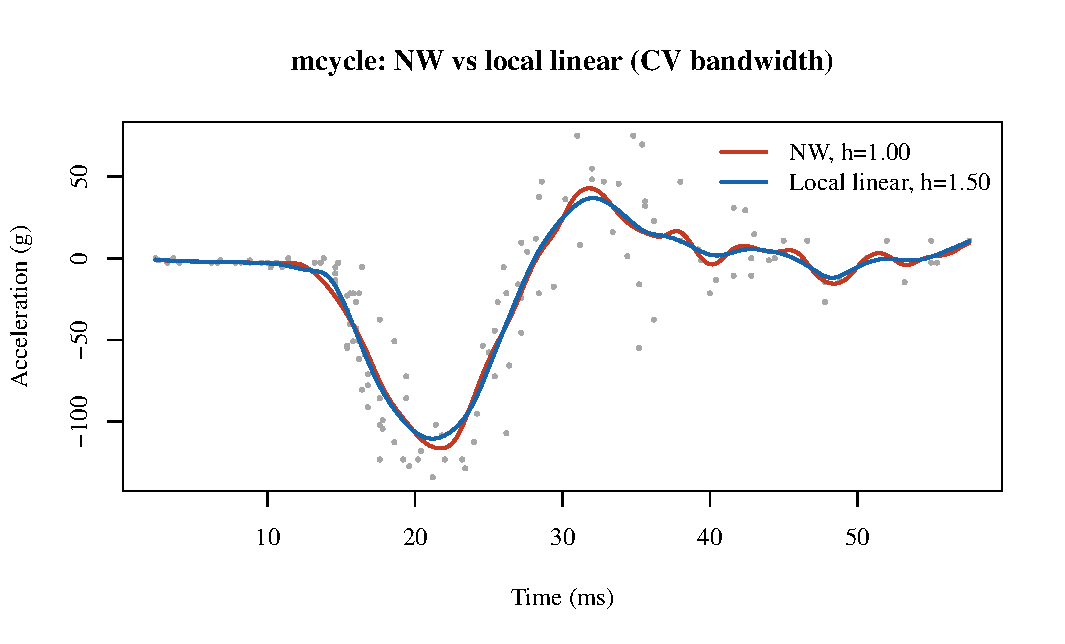
\includegraphics[width=.82\linewidth]{Final_Exam_Regression_Exercise7.pdf}
\end{center}
Mã slide 28 bỏ mọi quan sát có $X_j=X_i$;
nếu có thời gian trùng, điều đó bỏ nhiều hàng thay vì
đúng một hàng. Công thức ma trận trên chỉ bỏ quan sát
thứ $i$, đúng với leave-one-out.}

\stepdetail{85}{\par
Dưới đối xứng liên tục, $B_j$ độc lập
Bernoulli$(1/2)$ và
$W^+=\sum_{j=1}^n jB_j$.
Đặt $Z_j=j(B_j-1/2)$; khi đó
$\E Z_j=0$, $\Var Z_j=j^2/4$ và
$\E|Z_j|^3=j^3/8$.
Tổng phương sai
$s_n^2=\frac14\sum_{j=1}^n j^2\asymp n^3$,
nên $s_n^3\asymp n^{9/2}$.
Mặt khác $\sum_j\E|Z_j|^3=\frac18\sum_jj^3=O(n^4)$.
Vì vậy tỷ số Lyapunov bậc 3 là
\[
\frac{\sum_j\E|Z_j|^3}{s_n^3}
=O(n^{-1/2})\longrightarrow0.
\]
Định lý CLT Lyapunov cho
\[
\boxed{\frac{W^+-n(n+1)/4}
{\sqrt{n(n+1)(2n+1)/24}}
\Rightarrow N(0,1).}
\]
Đây là chứng minh hệ quả chuẩn tiệm cận phát biểu
ở trang 17, dưới giả thiết không có hạng trùng.}

\stepdetail{86}{\par
Ví dụ Spearman có $n=8$ và
$\sum_i(R_i-S_i)^2=4$, nên $\rho_S=20/21$.
Dưới $H_0$ độc lập với biên liên tục, mọi hoán vị
của hạng $1,\ldots,8$ đều xác suất $1/8!$.
Điều kiện $\rho_S\ge20/21$ tương đương
$\sum_i(i-\pi(i))^2\le4$.
Có 1 hoán vị đồng nhất (tổng 0), 7 phép đổi chỗ
hai hạng kề nhau (tổng 2), và
$\binom72-6=15$ cách đổi hai cặp kề nhau rời nhau
(tổng 4). Không còn dạng khác với tổng không quá 4.
Vậy một đuôi có $1+7+15=23$ hoán vị; đối xứng
cho hai đuôi $46$ hoán vị:
\[
\boxed{p_{\rm Spearman}=\frac{46}{8!}
\approx0.001141.}
\]
Slide 33 ghi $0.0003$, không khớp phép đếm chính xác.
Slide 33 ghi ngưỡng $0.714$ cho $n=8$, còn phụ lục
trang 43 ghi $0.738$; cả hai đều nhỏ hơn $20/21$,
nên quyết định bác bỏ ở $5\%$ không đổi.
Với Kendall, xếp theo $X$ thì dãy $Y$ ở slide 35 là
$(4,5.5,5,6,7.5,8.5,8,9)$.
Chỉ có hai cặp nghịch hành: $(5.5,5)$ và $(8.5,8)$.
Do đó $n_d=2$, $n_c=28-2=26$ và $\tau=6/7$.
Số hoán vị 8 phần tử có 0, 1, 2 nghịch thế lần lượt
là $1,7,27$; hai phía có $2(1+7+27)=70$ hoán vị.
\[
\boxed{p_{\rm Kendall}=\frac{70}{8!}
\approx0.001736,}
\]
khớp $0.0017$ làm tròn trên slide 36.}

\stepdetail{87}{\par
Taylor tại $x$ cho
\[
r(x+hz)=\sum_{k=0}^{\ell}
\frac{r^{(k)}(x)h^k}{k!}z^k+R_\ell.
\]
Nếu dùng cơ sở trang 30
$V_\ell(z)=(1,z,z^2/2!,\ldots,z^\ell/\ell!)^\top$,
thì tích vô hướng $\theta^\top V_\ell(z)$ khớp Taylor khi
\[
\boxed{\theta_k=r^{(k)}(x)h^k,
\qquad r^{(k)}(x)=\theta_k/h^k}
\quad(k=0,\ldots,\ell).
\]
Nếu đổi sang đơn thức thô $(X_i-x)^k$ như trang 32,
hệ số tương ứng là
$\beta_k=r^{(k)}(x)/k!$, nên
$r^{(k)}(x)=k!\beta_k$.
Hai tham số hóa cho cùng hệ số hằng $r(x)$.
Trang 42 viết thêm $/k!$ trong công thức cho $\theta_k$
dù trang 30 đã đặt $1/k!$ vào $V_\ell$;
không được chia factorial hai lần.}

\stepdetail{88}{\par
Từ cận ở trang 42, đặt
$M(h)=Ah^{2\beta}+B/(nh)$ với $A,B>0$.
Đạo hàm theo $h$:
\[
M'(h)=2\beta Ah^{2\beta-1}-\frac{B}{nh^2}.
\]
Giải $M'(h)=0$:
\[
\boxed{h_*^{2\beta+1}=\frac{B}{2\beta An},
\qquad h_*\asymp n^{-1/(2\beta+1)}.}
\]
Thế lại, hai hạng bias bình phương và phương sai
đều có bậc $n^{-2\beta/(2\beta+1)}$, nên
\[
\boxed{\operatorname{MSE}(h_*)
=O\!\left(n^{-2\beta/(2\beta+1)}\right).}
\]
Đây là \emph{cận trên} chứng minh bằng tối ưu hóa.
Slide 43 gọi tốc độ minimax tối ưu; để chứng minh chữ
``minimax'' còn cần cận dưới cho mọi estimator,
không được suy ra chỉ từ đạo hàm trên.}

\stepdetail{89}{\par
Ba thống kê nguyên trên slide có các tham số dưới $H_0$:
\[
\begin{array}{c|c|c}
T&\mu_0&\sigma_0^2\\\hline
S^+&n/2&n/4\\
W^+&n(n+1)/4&n(n+1)(2n+1)/24\\
U&nm/2&nm(n+m+1)/12
\end{array}
\]
Với một thống kê nguyên $T$, xấp xỉ chuẩn có
hiệu chỉnh liên tục cho hai đuôi là
\[
\PP_0(T\le t)\approx
\Phi\!\left(\frac{t+0.5-\mu_0}{\sigma_0}\right),
\qquad
\PP_0(T\ge t)\approx
1-\Phi\!\left(\frac{t-0.5-\mu_0}{\sigma_0}\right).
\]
Với kiểm định hai phía đối xứng, đặt
$d=|t-\mu_0|$ và lấy
\[
p\approx 2\left[1-\Phi\!\left(
\frac{d-0.5}{\sigma_0}\right)\right],
\]
cắt về $[0,1]$ nếu cần. Công thức trang 9 cho
kiểm định dấu chính là chuẩn hóa này.
Trang 18 ghi $-0.5$ trong $Z$ của $W^+$;
dấu ấy phù hợp với \emph{đuôi phải}; đuôi trái dùng
$+0.5$ theo công thức đầu. Với mẫu nhỏ, ưu tiên
phân phối nhị thức hoặc hoán vị chính xác trên slide.}

\stepdetail{90}{\par
Sắp mẫu theo thứ tự đã cho:
$1<1.2<1.5<2<2.5$, nên $n=5$ và mỗi quan sát
đóng góp $1/5$ vào ECDF khi $x$ đi qua nó.
Đếm số quan sát không vượt quá $x$ trên từng khoảng:
\[
\Fn(x)=\begin{cases}
0,&x<1,\\
1/5,&1\le x<1.2,\\
2/5,&1.2\le x<1.5,\\
3/5,&1.5\le x<2,\\
4/5,&2\le x<2.5,\\
1,&x\ge2.5.
\end{cases}
\]
Chẳng hạn $\Fn(1.5-)=2/5$, $\Fn(1.5)=3/5$,
nên bước nhảy tại $1.5$ là $1/5$; các điểm còn lại
cũng có bước nhảy $1/5$ vì mẫu không trùng.
Khoảng $(1.2,2]$ chứa $1.5$ và $2$, do đó
\[
\boxed{\widehat P((1.2,2])
=\Fn(2)-\Fn(1.2)=4/5-2/5=2/5.}
\]
Nếu lấy $[1.2,2]$ thì còn thêm quan sát $1.2$,
và phải dùng $\Fn(2)-\Fn(1.2-)=3/5$.}

\stepdetail{91}{\par
Vì $X_i\sim U[0,2]$, với $x_0=0.8$ ta có
\[
p=F(0.8)=\PP(X_i\le0.8)=\frac{0.8-0}{2-0}=0.4.
\]
Đặt $I_i=\mathbf1_{\{X_i\le0.8\}}$;
$I_i$ độc lập Bernoulli$(0.4)$ và
$100\Fn(0.8)=\sum_{i=1}^{100}I_i\sim\operatorname{Bin}(100,0.4)$.
Với $k=0,1,\ldots,100$,
\[
\PP\!\left(\Fn(0.8)=\frac{k}{100}\right)
=\binom{100}{k}(0.4)^k(0.6)^{100-k}.
\]
Vậy
\[
\E\Fn(0.8)=0.4,\quad
\Var\Fn(0.8)=\frac{0.4(0.6)}{100}=0.0024,
\quad \operatorname{SD}\Fn(0.8)=\sqrt{0.0024}\approx0.04899.
\]
$0.4$ là giá trị thật $F(0.8)$;
$\Fn(0.8)$ vẫn ngẫu nhiên trước khi quan sát mẫu.}

\stepdetail{92}{\par
Giả sử mẫu quan sát cho $\widehat p=0.4$ với $n=100$.
Với mức tin cậy $95\%$, $z_{0.975}\approx1.96$.
Sai số chuẩn cắm vào của Wald là
\[
\widehat{\operatorname{se}}
=\sqrt{\frac{0.4(1-0.4)}{100}}
=\sqrt{0.0024}\approx0.04899.
\]
Nửa độ rộng Wald là $1.96(0.04899)\approx0.09602$;
do đó
\[
\boxed{I_{\rm Wald}
=[0.4-0.09602,\,0.4+0.09602]
\approx[0.304,0.496].}
\]
Với Hoeffding, đặt $\alpha=0.05$:
\[
2e^{-2(100)\varepsilon^2}=0.05
\Longleftrightarrow
\varepsilon=\sqrt{\frac{\log(2/0.05)}{200}}
=\sqrt{\frac{\log40}{200}}\approx0.13581.
\]
Vì vậy
\[
\boxed{I_{\rm Hoeffding}
=[0.4-0.13581,\,0.4+0.13581]
\approx[0.264,0.536].}
\]
Wald hẹp hơn trong ví dụ này nhưng chỉ có độ phủ
xấp xỉ tiệm cận. Hoeffding bảo đảm độ phủ ít nhất
$95\%$ ở mọi cỡ mẫu cho một $x_0$ cố định.
Slide 21 viết $\widehat p=F(0.8)=0.4$;
đúng hơn là $F(0.8)=0.4$ trong mô hình và
$\widehat p=0.4$ chỉ khi mẫu quan sát cho tần suất ấy.}

\stepdetail{93}{\par
Với $x\ge0$, giải phương trình $u=F(x)$:
\begin{align*}
u&=1-e^{-\lambda x},\\
1-u&=e^{-\lambda x},\\
\log(1-u)&=-\lambda x,\\
x&=-\frac{\log(1-u)}{\lambda}.
\end{align*}
Lấy $U\sim U(0,1)$ rồi đặt
$X=-\log(1-U)/\lambda$. Với $x<0$, $\PP(X\le x)=0$.
Với $x\ge0$,
\begin{align*}
\PP(X\le x)
&=\PP\!\left(-\log(1-U)\le\lambda x\right)\\
&=\PP\!\left(U\le1-e^{-\lambda x}\right)\\
&=1-e^{-\lambda x}=F(x).
\end{align*}
Đó là kiểm tra trực tiếp của thuật toán mô phỏng
ở slide 9; $\lambda>0$ và $U=1$ có xác suất 0.}

\stepdetail{94}{\par
Chạy đúng thiết lập slide 26:
$X_i\sim U[0,1]$, $r(x)=\sin(2\pi x)+0.5x$,
$Y_i=r(X_i)+\xi_i$, $\xi_i\sim N(0,0.25^2)$,
$n=200$, \texttt{set.seed(2025)}.
Mã tái lập trong tệp
\begin{center}
\texttt{Final\_Exam\_Regression\_SlideSimulation.R}
\end{center}
Trang 27 so ba giá trị băng thông của
\texttt{ksmooth}: $0.02,0.08,0.30$.
Trang 28 tính CV của NW trên 40 giá trị từ $0.01$
đến $0.30$. Với mỗi $h$ và mỗi $i$, bỏ hàng thứ $i$,
tính $\widehat r_{-i,h}(X_i)$, rồi lấy
\[
\operatorname{CV}(h)
=\frac1{200}\sum_{i=1}^{200}
[Y_i-\widehat r_{-i,h}(X_i)]^2.
\]
Chạy theo seed và lưới trên cho
$\boxed{h_{\rm CV}\approx0.02487179}$,
$\min\operatorname{CV}\approx0.06163277$.
Chẳng hạn với quan sát thứ nhất,
$X_1\approx0.00459119$, $Y_1\approx0.20374538$.
Tại băng thông chọn được, bỏ hàng này cho
$\widehat r_{-1,h_{\rm CV}}(X_1)\approx0.10705432$.
Hạng thứ nhất của tổng CV là
\[
(0.20374538-0.10705432)^2\approx0.00934916.
\]
Ở $x=0$ với NW và $h=0.10$,
\[
\sum_i K((X_i-0)/h)Y_i\approx4.70238791,\qquad
\sum_i K((X_i-0)/h)\approx9.23387630,
\]
cho $\widehat r_{NW}(0)\approx4.70238791/9.23387630
=0.50925394$.
Với local linear $h=0.05$ tại cùng điểm,
\[
\begin{aligned}
(S_0,S_1,S_2)&\approx(3.66315099,0.14466935,0.01083560),\\
(T_0,T_1)&\approx(0.93056722,0.06295645).
\end{aligned}
\]
Vậy tử $S_2T_0-S_1T_1\approx0.00097538$,
mẫu $S_0S_2-S_1^2\approx0.01876320$,
và $\widehat r_{LL}(0)\approx0.05198375$.
Ở ba điểm kiểm tra, hàm thật và hai ước lượng
theo công thức Gaussian của slide cho
\[
\begin{array}{c|rrr}
x&r(x)&\widehat r_{NW,h=0.10}(x)
&\widehat r_{LL,h=0.05}(x)\\\hline
0&0&0.50925&0.05198\\
0.5&0.25&0.26258&0.28903\\
1&0.5&-0.01299&0.55408
\end{array}
\]
Tại $x=0$ và $x=1$, local linear gần $r(x)$ hơn
trong lần mô phỏng này; tại $x=0.5$ cả hai gần nhau.
\begin{center}
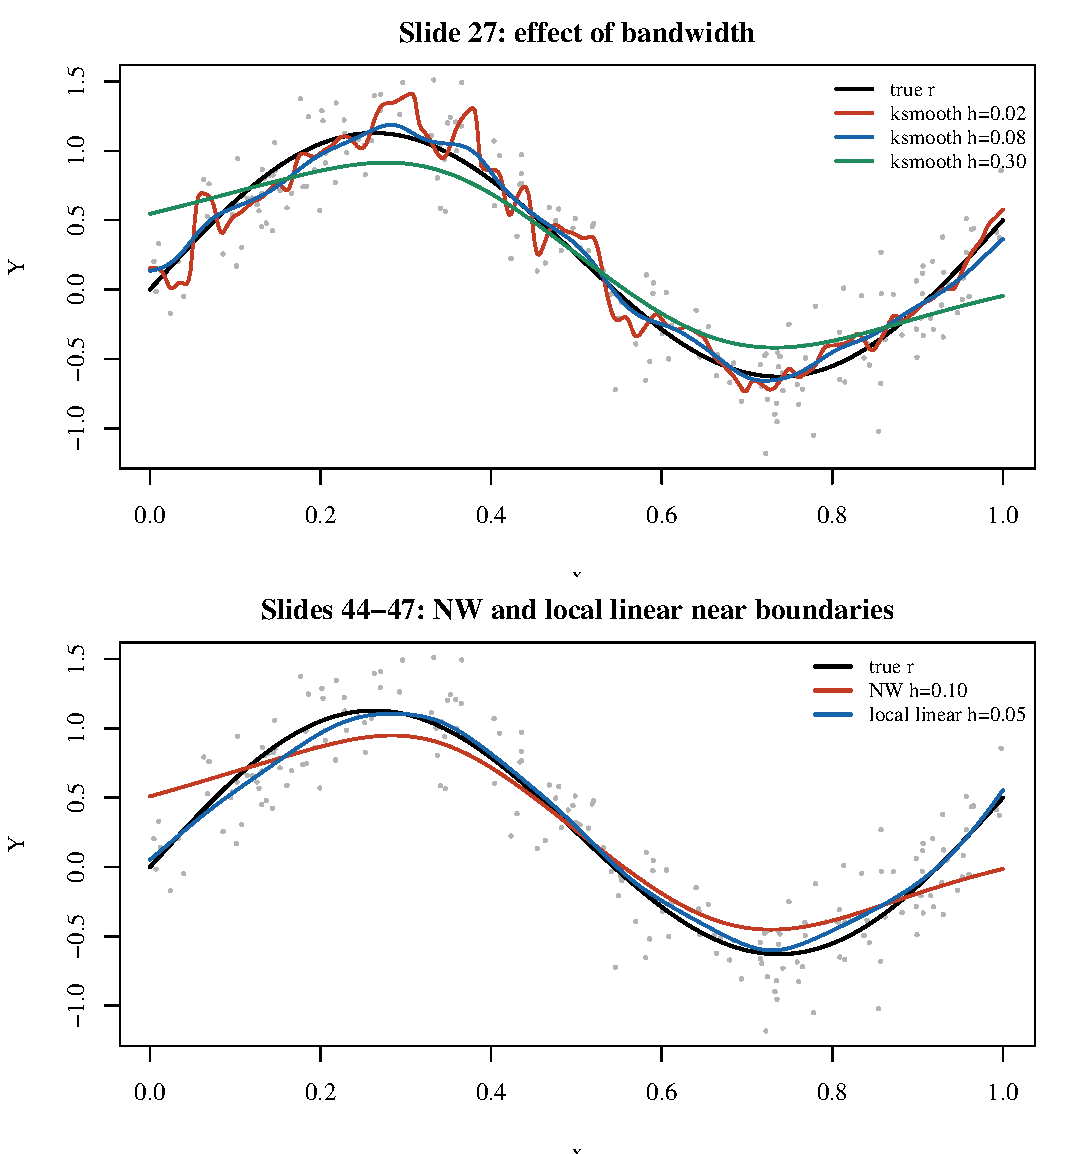
\includegraphics[width=.85\linewidth]{Final_Exam_Regression_SlideSimulation.pdf}
\end{center}
\texttt{ksmooth} ở trang 27 và công thức
\texttt{dnorm((X-x)/h)} ở trang 28 dùng hai cách
diễn giải đối số băng thông trong R;
vì thế không so trực tiếp số $0.08$ trên hình với
$h_{\rm CV}$ của công thức NW tự viết.}

\stepdetail{95}{\par
Trên slide, $X_i\sim N(4,25)$ và $n=1000$.
Mật độ thật là
\[
f(x)=\frac1{5\sqrt{2\pi}}
\exp\!\left[-\frac{(x-4)^2}{50}\right],
\qquad
\boxed{f(4)=\frac1{5\sqrt{2\pi}}\approx0.07979.}
\]
Từ mẫu, tính $a=\min_iX_i$, $b=\max_iX_i$
rồi $U_i=(X_i-a)/(b-a)$. Trên $[0,1]$,
\[
\widehat a_1=1,\quad
\widehat a_{2k}=\frac{\sqrt2}{1000}
\sum_{i=1}^{1000}\cos(2\pi kU_i),\quad
\widehat a_{2k+1}=\frac{\sqrt2}{1000}
\sum_{i=1}^{1000}\sin(2\pi kU_i).
\]
Thế hệ số $k=1$ cho $\widehat f_3$;
thêm $k=2$ cho $\widehat f_5$.
Với histogram $D=10$, đếm
$Y_j=\#\{i:U_i\in[(j-1)/10,j/10)\}$
(ô cuối nhận $U_i=1$) và đặt
$\widehat f_{10}(u)=10Y_j/1000$ trên ô $j$.
Cuối cùng, mọi mật độ ước lượng trên thang $x$ là
$\widehat f_{D,X}(x)=\widehat f_D((x-a)/(b-a))/(b-a)$.
Slide không công bố 1000 giá trị $X_i$ hoặc seed,
nên không thể tính số cụ thể của $a,b,\widehat a_j,Y_j$
hay giá trị $\widehat f_D(4)$ từ slide;
nhận xét $D=3$ quá trơn, $D=5$ khớp hơn và
histogram $D=10$ gián đoạn là đánh giá từ hình minh họa.}

\stepdetail{96}{\par
Sắp sáu quan sát tăng dần:
\[
1<2<3<5<6<8.
\]
Gán hạng theo thứ tự này: $1\mapsto1$,
$2\mapsto2$, $3\mapsto3$, $5\mapsto4$,
$6\mapsto5$, $8\mapsto6$.
Trả lại thứ tự ban đầu $(5,2,6,3,8,1)$:
\[
\boxed{(R_1,\ldots,R_6)=(4,2,5,3,6,1).}
\]
Kiểm tra $\sum_iR_i=4+2+5+3+6+1=21=6\cdot7/2$.
Ví dụ không có giá trị trùng nên không cần midrank.}

\stepdetail{97}{\par
Với $X\sim U[0,1]$, độ dài đoạn $[0,x]$ trong
$[0,1]$ là $x$ khi $0\le x\le1$, nên
\[
F_U(x)=\begin{cases}
0,&x<0,\\x,&0\le x\le1,\\1,&x>1.
\end{cases}
\]
Với $X\sim\operatorname{Exp}(0.5)$, mật độ là
$0.5e^{-0.5x}$ cho $x\ge0$; tích phân từ 0 đến $x$
cho
\[
F_E(x)=\begin{cases}
0,&x<0,\\1-e^{-0.5x},&x\ge0.
\end{cases}
\]
Với biến hỗn hợp, gọi $B=1$ nếu ta chọn khối điểm
$0.5$, $\PP(B=1)=1/2$; nếu $B=0$, lấy $U\sim U[0,1]$.
Theo công thức xác suất toàn phần,
\[
F_M(x)=\tfrac12\mathbf1_{\{x\ge0.5\}}
+\tfrac12F_U(x)
=\begin{cases}
0,&x<0,\\
x/2,&0\le x<0.5,\\
(1+x)/2,&0.5\le x\le1,\\
1,&x>1.
\end{cases}
\]
Vì $F_M(0.5-)=0.25$ và $F_M(0.5)=0.75$,
\[
\boxed{\PP(X=0.5)=F_M(0.5)-F_M(0.5-)=0.5.}
\]
Ví dụ này cho thấy CDF tồn tại dù phân phối vừa có
khối điểm vừa có phần liên tục.}

\stepdetail{98}{\par
Phân phối thực nghiệm đặt khối lượng $1/n$ tại mỗi $X_i$.
Vì thế, với mọi $g$ tính được tại các quan sát,
\[
\int g(x)\,d\Fn(x)=\frac1n\sum_{i=1}^ng(X_i).
\]
Thay lần lượt các hàm $g$ của slide 29:
\begin{align*}
\widehat\mu&=\int x\,d\Fn=\frac1n\sum_iX_i=\bar X,\\
\widehat m_k&=\int x^k\,d\Fn=\frac1n\sum_iX_i^k,\\
\widehat P(X>c)&=\int\mathbf1_{\{x>c\}}\,d\Fn
=\frac{\#\{i:X_i>c\}}n=1-\Fn(c),\\
\widehat F(t)&=\int\mathbf1_{\{x\le t\}}\,d\Fn
=\frac{\#\{i:X_i\le t\}}n=\Fn(t).
\end{align*}
Với phiếm hàm phi tuyến ở slide 30, trước hết tính
$\bar X$ và $\widehat m_2$, rồi
\[
\widehat\sigma^2=\widehat m_2-\bar X^2
=\frac1n\sum_i(X_i-\bar X)^2.
\]
Tiếp theo dùng moment trung tâm bậc ba:
\[
\widehat\kappa=
\frac{n^{-1}\sum_i(X_i-\bar X)^3}
{[n^{-1}\sum_i(X_i-\bar X)^2]^{3/2}},
\]
khi mẫu số dương. Với phân vị mức $p\in(0,1)$,
sắp mẫu và lấy
$\boxed{\widehat q_p=\Fn^{-1}(p)=X_{(\lceil np\rceil)}}$;
đặc biệt theo quy ước slide, median mẫu khi $n$ chẵn
là thống kê thứ tự thứ $n/2$, không lấy trung bình
hai giá trị giữa.
Nếu quan sát cặp $(X_i,Y_i)$, thay phân phối chung
bằng $P_n=n^{-1}\sum_i\delta_{(X_i,Y_i)}$.
Tính $\bar X,\bar Y$, hai phương sai và tích chéo:
\[
\widehat\rho=
\frac{\sum_i(X_i-\bar X)(Y_i-\bar Y)}
{\sqrt{\sum_i(X_i-\bar X)^2
\sum_i(Y_i-\bar Y)^2}},
\]
nếu cả hai phương sai dương. Các slide 29--35
không cho mẫu số liệu để thế thành giá trị cụ thể.}

\stepdetail{99}{\par
Hai hình ở slide 45 vẽ ECDF của nhóm $X$ và $Y$.
Ở hình trái, $F_X=F_Y$ dưới $H_0$;
hai đường thực nghiệm gần nhau nhưng vẫn có sai khác
do ngẫu nhiên hữu hạn mẫu. Ở hình phải, hai phân phối
khác nhau và khoảng cách giữa hai đường lớn hơn.
\begin{center}

\includegraphics[page=45,width=.84\linewidth]{../Slides/TKPTS_Chương 1.pdf}
\end{center}
Từ hai đường đó, trước hết tính
$\Delta(x)=\widehat F_X(x)-\widehat F_Y(x)$.
KS lấy độ lệch lớn nhất:
\[
T_{KS,2}=\sqrt{\frac{nm}{n+m}}\sup_x|\Delta(x)|.
\]
Đặt $\widehat H=(n\widehat F_X+m\widehat F_Y)/(n+m)$.
CvM cộng sai khác bình phương trên toàn miền,
còn AD tăng trọng số gần hai đuôi:
\[
T_{CvM,2}=\frac{nm}{n+m}\int\Delta(x)^2d\widehat H(x),
\quad
T_{AD,2}=\frac{nm}{n+m}\int
\frac{\Delta(x)^2}{\widehat H(x)(1-\widehat H(x))}
d\widehat H(x).
\]
Hình không liệt kê các $X_i,Y_i$ và không có ngưỡng
hay $p$-giá trị, nên không thể tính ba thống kê ra số
hoặc kết luận kiểm định chính thức chỉ từ hình minh họa.}

\stepdetail{100}{\par
Dùng đúng mẫu mô phỏng seed 2025 của slide 26.
Chạy $\texttt{KernSmooth::locpoly}$ với
\texttt{degree=1} và \texttt{degree=2},
cùng \texttt{bandwidth=0.08} như slide 45;
đặt lưới dự đoán từ 0 đến 1. Giá trị tại ba điểm là
\[
\begin{array}{c|rrr}
x&r(x)&\text{local linear}&\text{local quadratic}\\\hline
0&0&0.07221&0.05169\\
0.5&0.25&0.28226&0.27732\\
1&0.5&0.45877&0.58559
\end{array}
\]
Ví dụ ở $x=0$, sai số tuyệt đối lần lượt là
$|0.07221-0|=0.07221$ và $|0.05169-0|=0.05169$;
ở $x=1$, chúng là $0.04123$ và $0.08559$.
Vì vậy bậc 2 không thắng ở mọi điểm trong lần mô phỏng này;
đồ thị cho thấy nó theo sát vài đoạn cong hơn nhưng
cũng dao động hơn.
\begin{center}
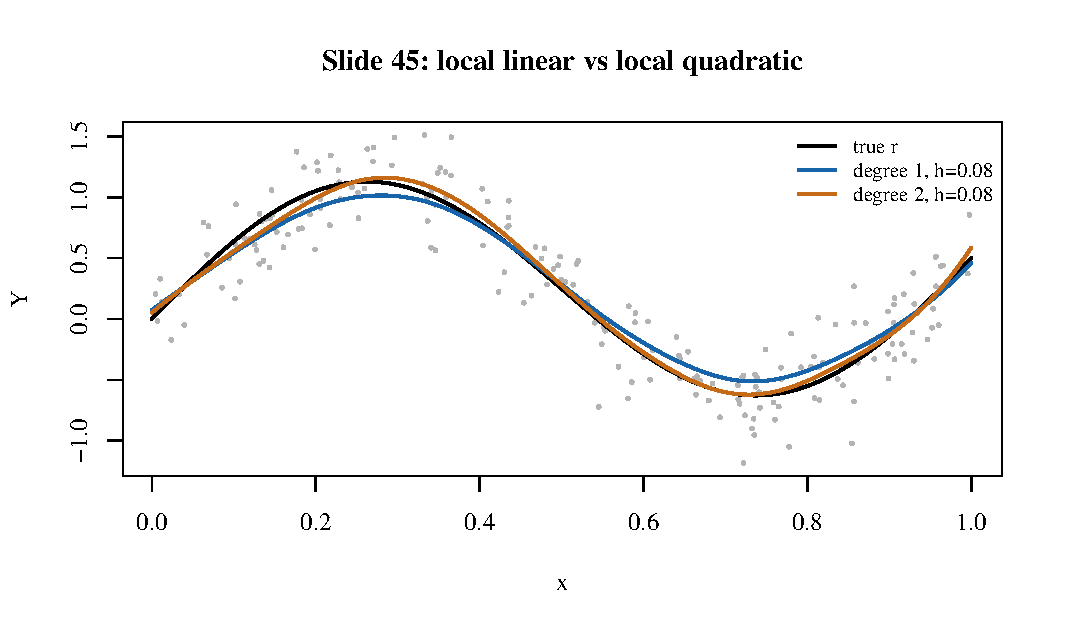
\includegraphics[width=.82\linewidth]
{Final_Exam_Regression_LocalPolynomials.pdf}
\end{center}
Hai đường dùng cùng dữ liệu và cùng đối số băng thông,
nên sự khác biệt ở đây đến từ bậc đa thức.
Mã tái lập nằm trong
\texttt{Final\_Exam\_Regression\_SlideSimulation.R}.}
